\tikzstyle{mybox} = [draw=gray, fill=gray!10, very thick,
rectangle, rounded corners, inner sep=10pt, inner ysep=20pt]
% Da aggiungere al preambolo?
\chapter{Limiti e colimiti}\label{chap_limiti_colimiti}
\epigraph{Più recentemente, la ricerca degli universali ha assunto anche una svolta concettuale, nella forma della Teoria delle Categorie.}{F.\ W.\ Lawvere, \cite{lawvere1969adjointness}}
\section{Tre versioni sui limiti}
Anche questo capitolo inizia raccogliendo degli esempi che la nozione di limite e di colimite organizzeranno come casi particolari di una stessa teoria, al cui cuore sta la nozione di \emph{proprietà universale}. Essa si riassume in modo estremamente conciso, mediante le nozioni di inizialità e terminalità che sono già state accennate rapidamente in \ref{def_cono_su_C}:
\begin{definition}\index{Oggetto!---	iniziale}\index{Oggetto!--- terminale}
	Sia \(\ctC\) una categoria. Un oggetto \(\init_\ctC\in\ctC_0\) si dice \emph{iniziale} in \(\ctC\) se soddisfa la seguente proprietà:
	\begin{quote}
		Per ogni \(C\in\ctC_0\), esiste una e una sola freccia \(\init_\ctC \to C\).
	\end{quote}
	Dualmente, un oggetto \(\term_\ctC\in\ctC_0\) si dice \emph{terminale} in \(\ctC\) se soddisfa la seguente proprietà:
	\begin{quote}
		Per ogni \(C\in\ctC_0\), esiste una e una sola freccia \(C\to\term_\ctC\).
	\end{quote}
\end{definition}
\begin{lemma}\label{init_ha_solo_id}
	Sia \(\ctC\) una categoria. Se \(\term\) è un oggetto terminale, l'unica freccia \(\term\to\term\) è l'identità \(\id_{\term}\). Se \(\init\) è un oggetto iniziale, l'unica freccia \(\init\to\init\) è l'identità \(\id_{\init}\).
\end{lemma}
\begin{proof}
	Evidentemente, deve esistere \emph{almeno} l'identità \(\id_{\term} : \term\to\term\), e del resto non può esistere nessun'altra freccia. Del tutto analoga è la dimostrazione per \(\init\).
\end{proof}
La natura duale dei due enunciati che compongono \ref{init_ha_solo_id} è un fatto molto generale. Evidentemente, la proprietà di essere iniziale in \(\ctC\) è precisamente la proprietà di essere terminale in \(\ctC^\op\), e viceversa, la proprietà di essere terminale in \(\ctC\) è precisamente la proprietà di essere iniziale in \(\ctC^\op\). La maggior parte dei risultati che vedremo nel capitolo sono dualizzabili; per ragioni pedagogiche insisteremo a enunciare le due forme duali dei primi risultati per poi lasciare la dualizzazione come un (quasi sempre semplice) esercizio per chi legge. Imparare a dualizzare un enunciato, e a farlo correttamente (si veda \ref{ocio_al_duale}), è una parte inevitabile del percorso di apprendimento di chi studia la teoria delle categorie.
\paragraph*{Proprietà universali.}\index{Proprietà!--- universale}\index{Proprietà!--- couniversale}
In maniera molto informale, si dice \emph{universale} la proprietà di essere terminale in una opportuna categoria, e dualmente avere una proprietà \emph{couniversale} significa essere iniziale.

Chiaramente questo è impreciso (gli oggetti sono sempre tipati dalla categoria cui appartengono, si veda la nota \ref{fn_tipati} a pagina \pageref{fn_tipati} nel capitolo precedente), e fuorviante se preso troppo alla lettera; si dovrebbe dire che un oggetto \(X\in\ctC_0\) è universale in \(\ctC\) quando è possibile costruire un certo diagramma, e da esso un `cono' la cui `origine' è \(X\), la cui forma somiglia a
\begin{equation}\label{cone}\vcenter{\xymatrix@R=0mm{
	& Di \\
	X \ar@{->}[ru] \ar@{->}[r] \ar@{->}[rdd] & Dj \\
	& \vdots \\
	& Dk
	}}
\end{equation}
che è terminale in una categoria i cui oggetti sono questi `coni' della stessa forma. Al variare del diagramma \(D\) (quanto è complesso il suo dominio, quanto è complessa la sua azione su oggetti e frecce dello stesso), varia la complessità interna dell'oggetto terminale, che riesce a descrivere oggetti molto strutturati (i nuclei di omomorfismi, si veda \ref{ex_lim_kernel}; i grafici di funzioni reali o complesse, si veda \ref{ex_lim_grafici}; ma anche i numeri \(p\)-adici, si veda \ref{ex_lim_padici}; alcuni frattali, si veda \ref{ex_lim_frattali}; etc). L'oggetto \(X\) si dice allora il \emph{limite} del diagramma \(D\).

Dualmente, un oggetto \(X\in\ctC_0\) è \emph{co}universale in \(\ctC\) quando è il bersaglio di un \emph{co}cono \emph{iniziale},
\begin{equation}\label{cocone}\vcenter{\xymatrix@R=0mm{
	Di \ar@{->}[rd] &  \\
	Dj \ar@{->}[r] & X \\
	\vdots &  \\
	Dk \ar@{->}[ruu] &
	}}\end{equation}
ossia di un oggetto iniziale in una categoria di coconi per \(D\). L'oggetto \(X\) si dice allora il \emph{colimite} del diagramma \(D\). Anche i colimiti riescono a descrivere oggetti molto strutturati (i numeri naturali, si veda \ref{ex_colim_nat}; i prodotti liberi di gruppi e monoidi, si veda \ref{ex_colim_liberi}; le liste a valori in un alfabeto \(S\), si veda \ref{ex_colim_liste}; i cosiddetti \emph{catamorfismi}, si veda \ref{ex_colim_cata};\dots).
\paragraph*{Problemi di minimo-massimo.}
Il punto di vista appena esposto, seppure profondamente utile, tuttavia non è l'unico, né il più pedagogicamente efficace in assoluto. Sarebbe altrettanto valido introdurre la nozione di limite e di colimite come `soluzione' a un problema di `ottimizzazione', o di minimo-massimo:
\begin{itemize}\index{Estremo inferiore}\index{Estremo superiore}
	\item Il limite del diagramma \(D : \ctJ\fun\ctC\) è il `massimo dei minoranti' tra diagrammi della forma \eqref{cone} (dove le frecce sono disuguaglianze); in effetti, in un insieme ordinato (che sappiamo essere una categoria per \ref{ord_sonocat}), l'estremo inferiore di un sottoinsieme \(S\subseteq P\) è un elemento \(\inf S\) con la proprietà
	      \[\forall s\in S : \inf S \le s\qquad \forall s\in S : y\le s \Rightarrow y\le \inf S\]
	\item Dualmente, il colimite del diagramma \(D : \ctJ\fun\ctC\) è il `minimo dei maggioranti' tra diagrammi della forma \eqref{cocone} (dove le frecce sono disuguaglianze); in effetti, in un insieme ordinato l'estremo superiore di un sottoinsieme \(S\subseteq P\) è un elemento \(\sup S\) con la proprietà
	      \[\forall s\in S : s\le\sup S \qquad \forall s\in S : s\le y \Rightarrow \sup S\le y.\]
\end{itemize}
\begin{remark}
	Chi legge dovrebbe ricordare quando nei primissimi minuti di un corso di analisi è stata introdotta la proprietà dell'estremo superiore/inferiore per un sottoinsieme \(S\subseteq\bbR\); \emph{quella} è una particolare proprietà (co)universale.
\end{remark}
In ogni insieme ordinato, quindi, la nozione di (co)limite nella associata categoria-preordine si riduce alla proprietà dell'estremo superiore	o inferiore. La descrizione di limiti e colimiti in una categoria-preordine nel senso generale verrà delineata più in dettaglio in \ref{}, ma invitiamo già chi legge a immaginare come essa si possa sviluppare.\footnote{Un semplice esercizio per cui non serve alcun prerequisito	non elementare, è mostrare i fatti seguenti, che comunque verranno ripetuti più avanti: se \(\le\) è un preordine su \(P\), un oggetto iniziale della categoria \((P,\le)\) è un elemento \(\le\)-minimo di \(P\) o equivalentemente è, quando esiste, \(\sup \varnothing\); dualmente, un oggetto terminale di \((P,\le)\) è un elemento \(\le\)-massimo di \(P\), o equivalentemente è, quando esiste, \(\inf\varnothing\); se l'ordine è antisimmetrico, poi, \(\sup\varnothing\) e \(\inf\varnothing\) sono \emph{strettamente} unici quando esistono.}

La teoria dei limiti e dei colimiti si può vedere come la teoria di `estremi superiori e inferiori' per categorie che non sono preordini.

\medskip
Questa filosofia sui limiti tuttavia va al di là della `pura' teoria degli insiemi; la nozione di proprietà universale spiega infatti il motivo per cui (ad esempio) nel definire una topologia sul prodotto Cartesiano di due spazi \(X,Y\) la scelta `naturale' sia la topologia prodotto: non è una scelta di comodo né dettata dalla consuetudine, ma \emph{l'unica risposta giusta} se si desidera che lo \emph{spazio} \(X\times Y\) abbia la proprietà universale di un prodotto nella categoria \(\ctTop\). Allo stesso modo, la definizione di proprietà universale spiega
\begin{itemize}\index{Gruppo!--- topologico}\index{Limite!--- di catena}\index{Numeri \(p\)-adici}\index{aaa_Zp@\(\bbZ_p\)}
	\item il motivo per cui quando si definisce un `gruppo topologico' (per esempio i gruppi di Lie che sono ubiquitari in fisica matematica) le operazioni di gruppo, moltiplicazione e inversione, devono essere continue. \`E certamente una scelta `ovvia', ma essa è anche \emph{obbligata} dal fatto che la moltiplicazione deve essere una freccia della categoria \(\ctTop\ctGrp\), cioè \emph{sia} una freccia di \(\ctTop\), quando si dimentica la struttura di gruppo, sia una freccia di \(\ctGrp\), quando si dimentica la topologia;
	\item il motivo per cui su certi oggetti complicati, ad esempio il gruppo profinito degli interi \(p\)-adici (con \(p\) un numero primo) è il limite \(\bbZ_p\) della catena
	      \[\xymatrix{
		      0 & \ar[l]_-{\varphi_1} \bbZ/p\bbZ & \bbZ/p^2\bbZ \ar[l]_-{\varphi_2} & \bbZ/p^3\bbZ \ar[l]_-{\varphi_3} & \bbZ/p^4\bbZ \ar[l]_-{\varphi_4} & \cdots \ar[l]_-{\varphi_5}
		      }\]
	      dove ciascuna mappa \(\varphi_n : \bbZ/p^n\bbZ \to \bbZ/p^{n-1}\bbZ\) è la mappa di riduzione modulo \(p\), suriettiva e di nucleo \(p^{n-1}\bbZ/p^n\bbZ\); la topologia naturale su \(\bbZ_p\) (che lo rende uno \emph{spazio di Stone} oltre che un gruppo topologico) è universale a rendere continue tutte le proiezioni canoniche \(\bbZ_p \to \bbZ/p^n\bbZ\), e quindi che conferisce a \(\bbZ_p\) la proprietà universale di limite in \(\ctTop\); su certi oggetti quindi compare una topologia non discreta \emph{anche se tutte le componenti del diagramma sono spazi discreti}. Gli elementi di \(\bbZ_p\) si possono vedere come `serie di potenze nella variabile \(p\)' nel senso che un elemento \(x\in\bbZ_p\) è una successione	\(\overline x = (x_0,x_1,x_2,x_3\dots)\) tale che per ogni \(n\ge 0\) si abbia \(x_n\equiv x_{n+1}\pmod{p^n}\); del resto, se \(x_0 = k_0+x_1\), \(x_1 = k_1p+x_2\), \(x_2 = k_2p^2+x_3\), \dots, si ha che
	      \[\overline x \approx k_0 + k_1p + k_2p^2 + k_3p^3 + k_4p^4 + k_5p^5 + \dots \]
\end{itemize}
\paragraph*{Natura relazionale delle categorie.}
Uno dei paradigmi essenziali della teoria delle categorie vuole che, per indagare le proprietà di un determinato oggetto \(X\in\ctC_0\), si debba guardare al modo in cui esso interagisce con gli altri oggetti di \(\ctC\); anche questa è una maniera valida di introdurre la teoria dei limiti e dei colimiti, e lo scopo principale di questo capitolo sarà di conciliare queste tre prospettive.

Data una famiglia di oggetti di \(\ctC\), soggetta a determinate relazioni (il `diagramma'), si può trovare `l'oggetto più grande che è soluzione delle equazioni imposte dalla relazioni'? (E qual è il significato di questa qualificazione?) Dualmente: si può trovare `l'oggetto più piccolo in cui le equazioni imposte dalle relazioni sono verificate'?
\Todo{}
Esempi essenziali di limiti e colimiti nella categoria \(\ctSet\) di insiemi e funzioni coinvolgono le costruzioni fondamentali di \emph{sottoinsieme} e di \emph{insieme quoziente} (rispetto a una relazione di equivalenza):
\begin{itemize}\index{Equalizzatore}\index{Coequalizzatore}
	\item l'equalizzatore di due funzioni \(f,g : A \to B\), definito come
	      \[E(f,g) := \{ a \in A \mid fa = ga\} \subseteq A\]
	      che in virtù di questa definizione ha la proprietà per cui ogni funzione \(h : X \to A\) tale che \(f\cmp h = g\cmp h\) assume valori in \(E\), ciò si fattorizza in modo unico come
	      % https://q.uiver.app/#q=WzAsNCxbMCwxLCJFKGYsZykiXSxbMiwxLCJBIl0sWzEsMCwiWCJdLFszLDEsIkIiXSxbMiwxLCJoIl0sWzAsMSwiIiwyLHsic3R5bGUiOnsidGFpbCI6eyJuYW1lIjoiaG9vayIsInNpZGUiOiJ0b3AifX19XSxbMiwwLCJcXGJhciBoIiwyLHsic3R5bGUiOnsiYm9keSI6eyJuYW1lIjoiZG90dGVkIn19fV0sWzEsMywiZyIsMix7Im9mZnNldCI6Mn1dLFsxLDMsImYiLDAseyJvZmZzZXQiOi0yfV1d
	      \[\begin{tikzcd}
			      & X \\
			      {E(f,g)} && A & B
			      \arrow["{\bar h}"', dotted, from=1-2, to=2-1]
			      \arrow["h", from=1-2, to=2-3]
			      \arrow[hook, from=2-1, to=2-3]
			      \arrow["g"', shift right=1, from=2-3, to=2-4]
			      \arrow["f", shift left=1, from=2-3, to=2-4]
		      \end{tikzcd}\]
	\item il coequalizzatore di due funzioni \(f,g : A \to B\), definito considerando la relazione di equivalenza \(\sim_{f,g}\) su \(B\) generata dalle coppie \((fa,ga)\) per ogni \(a\in A\) (si veda \ref{rel_equiv_generata}), e ponendo poi \(Q(f,g) := B/_{\!\sim_{f,g}}\); per definizione, la proiezione canonica \(\pi : B \to Q(f,g)\) ha la proprietà seguente: ogni funzione \(h : B \to Y\) tale che \(h\cmp f = h\cmp g\) `scende al quoziente' (perché è costante sulle classi di equivalenza di \(\sim_{f,g}\)) si fattorizza in modo unico come
	      \[\begin{tikzcd}
			      & X \\
			      {Q(f,g)} && B & A
			      \arrow["{\bar h}"', dotted, to=1-2, from=2-1]
			      \arrow["h", to=1-2, from=2-3]
			      \arrow[two heads, to=2-1, from=2-3]
			      \arrow["g"', shift right=1, to=2-3, from=2-4]
			      \arrow["f", shift left=1, to=2-3, from=2-4]
		      \end{tikzcd}\]
\end{itemize}
Risulta allora evidente il senso di un'idea su esposta: l'equalizzatore di \(f,g\) consiste del più grande \emph{sottoinsieme} di \(A\) dove l'equazione \(f=g\) è valida. Invece, il coequalizzatore delle stesse \(f,g\) consiste del più piccolo \emph{quoziente} di \(B\) rispetto alla relazione più piccola dove viene imposta l'uguaglianza \(f=g\) (chi legge ed è familiare con la nozione di classe laterale, o con la più semplice definizione di spazio vettoriale quoziente, rifletta sul modo in cui \(V/W\) si realizza a questa maniera, e confronti \ref{quozienti_in_vect} con la sua idea). Limiti e colimiti sono nozioni duali; nella categoria degli insiemi, l'equalizzatore di due funzioni è un limite, e il coequalizzatore è un colimite. Dunque, fattorizzare una funzione attraverso un sottoggetto del suo codominio, e farla scendere ad un quoziente del suo dominio, sono in un certo senso operazioni duali.
\begin{remark}
	Una importante osservazione (che sebbene del tutto elementare, confonde molta gente\dots) è questa: ovviamente, il minimo sottoinsieme dove l'equazione \(f=g\) è valida è facile da determinare: è il vuoto, dove l'antecedente in \(\forall a\in\varnothing.(fa=ga)\) è banalmente vero. Altrettanto semplice è determinare il \emph{massimo} quoziente di \(B\) dove le immagini di \(f\) e \(g\) coincidono: è il quoziente banale \(B/_{\!\sim} = \singleton\) dove ogni elemento di \(B\) è equivalente a ogni altro elemento di \(B\). Perciò, queste due combinazioni di massimo/minimo e sottoinsieme/insieme quoziente non sono interessanti: vanno considerati \emph{tutti} gli elementi \(a\) tali che \(fa=ga\), e vanno identificati \emph{solo} gli elementi della chiusura riflessiva, simmetrica e transitiva di \((fa,ga)\subseteq B\times B\).
\end{remark}
\Todo{}
Questi, e molti altri concetti, appariranno più chiari quando avremo delineato la teoria generale.
\Todo{}
\begin{hExamples}[Alcuni esempi di oggetti iniziali e terminali]{fund}
	Raccogliamo alcuni esempi di oggetti iniziali e terminali in alcune categorie studiate nel capitolo precedente.
	\begin{enumtag}{it}
		\item\label{it_1} Nella categoria \(\ctSet\) di \ref{ex_cat_insiemi}, fatta da insiemi e funzioni, l'insieme vuoto \(\emptyset\) (senza elementi) è iniziale, dato che la condizione
		\[\forall S\in\ctSet_0 \text{ esiste uno e un solo sottoinsieme } f\subseteq \emptyset\times S \]
		è realizzata (banalmente) solo dall'insieme vuoto dato che \(\emptyset\times S = \emptyset\). Per contro, si osservi che una funzione \(S \to \emptyset\) esiste se e solo se \(S=\emptyset\). Ragionando in modo simile si ottiene che anche nella categoria di spazi topologici l'insieme vuoto \(\emptyset\), con l'unica topologia possibile, è un oggetto iniziale. Dualmente, ogni insieme \(\{\bullet\}\) che abbia un solo elemento è terminale, dato che per ogni \(S\in\ctSet_0\), esiste un'unica possibile funzione \(f : S \to \{\bullet\}\) che mappa tutto \(s\in S\) in \(\bullet\). Analogamente, nella categoria degli spazi topologici di \ref{}, per ogni spazio topologico \((X,\tau)\) esiste un'unica funzione continua \(X \to \{\bullet\}\) quando il codominio ha la topologia banale (che coincide con quella discreta).
		\item\label{it_2} Nella categoria di modelli di una segnatura algebrica \(\Sigma\) (come in \ref{}) che contiene solo una operazione binaria, l'insieme vuoto (definendo l'operazione come la funzione vuota) è un oggetto iniziale, e lo stesso accade se l'operazione è associativa o commutativa; le cose cambiano non appena la segnatura contiene una \emph{costante}, perché questo obbliga ogni modello a contenere una interpretazione di almeno quella costante, e quindi ogni supporto del modello deve contenere almeno un elemento (questo è il caso dei monoidi, dei gruppi, gruppi abeliani, insiemi puntati\dots --in questi ultimi l'unica operazione è proprio una costante). Nella categoria dei gruppi abeliani è il gruppo banale \(\init_\ctAb=\{0\}\) a essere iniziale, ma accade qualcosa di peculiare: \(\init_\ctAb\) è anche \emph{terminale} (è quello che si dice un \emph{oggetto zero}).
		\item\label{it_3} Nella categoria degli anelli unitari \(\ctRing_1\) di \ref{varie_categorie_nella_pratica} (in cui \(0\ne 1\) e gli omomorfismi rispettano entrambi, di modo che non esiste l'anello \(\{0\}\)), l'oggetto iniziale è l'anello degli interi \(\bbZ\): dato un anello unitario \(R\), un omomorfismo di anelli \(\varphi : \bbZ \to R\) deve mandare \(0\) in \(0_R\) e \(1\) in \(1_R\); del resto deve anche essere tale che \(\varphi(n) = \varphi(n\cdot 1) = n \cdot 1_R = \iter[1][+]1\) ed è quindi definito su tutti gli altri interi. Nella sottocategoria degli anelli con divisione, però, un oggetto iniziale non esiste: per quale motivo? (per chi vuole un suggerimento: se un oggetto iniziale esiste, quale ne deve essere la caratteristica?)
		\item\label{it_4} Nella categoria delle algebre di Boole di \ref{varie_categorie_nella_pratica}, l'oggetto iniziale è l'algebra con due elementi \(\bbB=\{\bot < \top\}\) (con le operazioni di congiunzione, disgiunzione e complemento usuali): se \(H\) è un'altra algebra di Boole, dato che un omomorfismo di algebre di Boole/Heyting deve mandare \(\bot\) in \(\bot\) e \(\top\) in \(\top\), deve esistere un unico \(\bang_H : \bbB \to H\). Un oggetto terminale è invece dato dall'algebra di Boole banale (con un solo elemento \(\bot=\top\)); sebbene l'interesse logico per un oggetto del genere sia praticamente nullo, questo è l'unico modo di garantire che per ogni algebra di Boole \(H\) esista un \emph{unico} omomorfismo \(H \to \term_\ctBAlg\). L'insieme \(\Hom{\ctBAlg}(H,\bbB)\) è interessante, ma lungi dall'essere un singoletto: si veda \ref{ex_21_1}.
		\item\label{it_5} Nella categoria dei sistemi dinamici di \ref{ex_cat_dyn} succede qualcosa di interessante, osservato nell'esercizio \ref{ex_monepi_3}: l'oggetto iniziale è il sistema dinamico \(\bsN=((\bbN,0),s)\) dove \(s : \bbN \to \bbN\) è la funzione successore \(n\mapsto 1+n\);
		%; infatti, 
		% \begin{itemize}
		per ogni sistema dinamico \(((X,x_0),f)\) esiste un unico omomorfismo \(u_f : \bbN \to X\), definito `per induzione' dalla regola
		\[u_f(0) := x_0 \qquad u_f(1+n) := f(u_f(n))\]
		che quindi evidentemente è definito in modo tale che
		\[\xymatrix{
				\singleton\ar[r]^{0}\ar[dr]_{x_0} & \bbN\ar[r]^s\ar[d]_{u_f} & \bbN \ar[d]_{u_f}\\
				& X \ar[r]_f & X
			}\]
		commuti in tutte le sue parti. Si noti che è essenziale che gli insiemi in questione siano puntati (quindi, non vuoti). Ammettendo sistemi dinamici con supporto vuoto, infatti, sarebbe l'insieme \(\emptyset\) (con l'unica azione possibile \(\id_\emptyset : \emptyset \emptyset\)) ad essere iniziale.
		% 	\item se esiste un altro	omomorfismo \(v : \bbN \to X\), per definizione si ha che \(v(0) = x_0\) e \(v(s(n))=v(1+n) = f(v(n))\); perciò, per induzione su \(n\), si ottiene che \(v(n) = u_f(n)\) per ogni \(n\in\bbN\), e quindi \(v = u_f\).
		% \end{itemize}
		\item\label{it_6} Data una categoria \(\ctC\), la categoria incubo \(\ctC/X\) sopra un oggetto possiede sempre un oggetto terminale, e la succuba sotto un oggetto \(X/\ctC\) possiede sempre un oggetto iniziale: la freccia identità di \(X\). Infatti (si ragiona dualmente per \(X/\ctC\)), se \(u : A \to X\) è un oggetto della categoria incubo su \(X\), la stessa \(u\) è l'unica freccia \(u : (A,u) \to (X,\id_X)\). Leggermente più in generale, un oggetto \(t : T \to X\) dell'incubo \(\ctC/X\) è terminale se e solo se \(t\) è un isomorfismo in \(\ctC\). In un verso, la cosa è ovvia. Di converso, se \(t\) come appena definito è terminale, allora esiste un'unica freccia \(k : X \to T\) tale che \(t\cmp k = \id_X\); quindi \(t\cmp k \cmp t = t\), e allora (per unicità) anche \(k\cmp t\) è uguale a \(\id_T\).
		\item\label{it_7} In un preordine guardato come categoria, un oggetto iniziale consiste di un elemento \(\bot\in P\) con la proprietà che per ogni \(x\in P\) si abbia \(\bot\le x\); quindi un oggetto iniziale è un elemento \emph{minimo}. Dualmente, un oggetto terminale è un massimo \(\top\), con la proprietà che per ogni \(x\in P\) si abbia \(x\le \top\). L'ordine stretto e totale \((\bbN,\le)\) ha iniziale/minimo ma non terminale/massimo, e altrettanto è vero per \(\bbR_\ge := [0,\infty)\); L'ordine stretto e totale \((\bbZ,\le)\) non ha né minimo né massimo; l'ordine di divisibilità \((\bbN,\div)\) accennato in \ref{alcuni_es_ordini} ha per oggetto iniziale \(1\) (ogni \(m\in\bbN\) è tale che \(m = 1\cdot m\)) e \(0\) per oggetto terminale (ogni \(m\in\bbN\) è tale che \(0 = m\cdot 0\)). L'ordine stretto e parziale sull'insieme delle parti \(PS\) di un insieme \(S\) ha il sottoinsieme vuoto come minimo/iniziale e il sottoinsieme \(S\subseteq S\) come massimo/terminale.
	\end{enumtag}
\end{hExamples}
\begin{lemma}\label{equivs_preservano_init_term}
	Se \((F,G,\eta,\epsilon):\ctC\simeq\ctD\) è un'equivalenza di categorie come in \ref{funtore_equcat}, e \(\init\in\ctC_0\) è un oggetto iniziale, allora \(F\init\in\ctD_0\) è un oggetto iniziale di \(\ctD\). Dualmente, se \(\term\in\ctC_0\) è un oggetto terminale, allora \(F\term\in\ctD_0\) è un oggetto terminale di \(\ctD\).

	Similmente, se \(\init\in\ctD_0\) è un oggetto iniziale, allora \(G\init\in\ctC_0\) è un oggetto iniziale di \(\ctC\), e se \(\term\in\ctD_0\) è un oggetto terminale, allora \(G\term\in\ctC_0\) è un oggetto terminale di \(\ctC\).
\end{lemma}
\begin{proof}
	Tutti e quattro gli enunciati si dimostrano allo stesso modo, \emph{mutatis mutandis}. Quindi dimostriamo solo il primo, e in effetti facciamo uso solo del fatto che \(F : \ctC \fun \ctD\) è un'equivalenza debole di categorie. In quanto tale, è pienamente fedele; allora, dato un oggetto \(D\in\ctD_0\), esiste un oggetto \(C\in\ctC_0\) tale che \(FC\) è isomorfo a \(D\), con un isomorfismo \(k : FC \cong D\). Dunque in \(\ctC\) esiste un'unica \(\bang_C : \init \to C\); ma allora,
	\begin{itemize}
		\item \(k\cmp F(\bang_C)\) è una freccia \(F\init \to FC \xto k D\);
		\item se si trova un altro oggetto \(C'\) con un isomorfismo \(h : FC'\cong D\), il quadrato
		      \[\xymatrix{
			      F\init\ar[r]^-{F\bang_C}\ar[d]_{F\bang_{C'}} & FC \ar[d]^k_\wr \\
			      FC' \ar[r]_-h^-\sim & D
			      }\]
		      sta nell'immagine di \(F\) (perché è pienamente fedele), ed è commutativo in \(\ctC\); allora è commutativo anche in \(\ctD\), di modo che fissato \(D\in\ctD_0\), per ogni \(C\in \ctC_0\) e ogni isomorfismo \(k : FC \cong D\), esiste un'unica freccia \(F\init\to D\).
	\end{itemize}
	Questo conclude la dimostrazione.
\end{proof}
I due esempi che seguono sono importanti per fissare l'idea in chi legge che un oggetto iniziale o terminale può essere `grande' o `complicato' e che sebbene la sua definizione sia semplice, in molti casi concreti la sua esistenza è un fatto altamente non banale.
\begin{proposition}\label{init_term_elements}
	Sia \(\ctC\) una categoria. Le condizioni seguenti sono equivalenti, per un funtore \(F : \ctC \fun\ctSet\):
	\begin{itemize}
		\item Esiste un isomorfismo naturale \(F\natIso \Hom{\ctC}(X_F,\blank)\) (cioè, nella terminologia di \ref{def_rappre_fun} \(F\) è corappresentabile da un oggetto \(X_F\));
		\item la categoria degli elementi \(\Elts{\ctC}F\) ha un oggetto iniziale \((\init,h\in F\init)\).
	\end{itemize}
	Dualmente, le condizioni seguenti sono equivalenti, per un funtore \(G : \ctC^\op \fun\ctSet\):
	\begin{itemize}
		\item Esiste un isomorfismo naturale \(G\natIso \Hom{\ctC}(\blank,Y_G)\) (cioè, nella terminologia di \ref{def_rappre_fun} \(G\) è rappresentabile da un oggetto \(Y_G\));
		\item la categoria degli elementi \(\Elts{\ctC}G\) ha un oggetto terminale \((\term,b\in G\term)\).
	\end{itemize}
\end{proposition}
\begin{proof}
	Dimostriamo la prima equivalenza, la seconda è duale.

	Se \(F\natIso \Hom{\ctC}(X_F,\blank)\), allora \(\Elts{\ctC}F\) è isomorfa alla categoria succuba \(X_F/\ctC\), che per \ref{elts_rappre} ha un oggetto iniziale \((X_F,\id_{X_F})\). Dunque, anche \(\Elts{\ctC}F\) ha un oggetto iniziale in virtù di \ref{equivs_preservano_init_term}.

	L'implicazione non ovvia è l'altra: supponiamo che \(\Elts{\ctC}F\) abbia un oggetto iniziale \((\init,h\in F\init)\), e ci proponiamo di costruire un isomorfismo naturale \(F\natIso \Hom{\ctC}(\init,\blank)\).
\end{proof}
\begin{proposition}\label{term_coalgebra_maybe}
	L'oggetto terminale della categoria delle \(S\)-coalgebre, dove \(S=1+(A\times\blank) : \ctSet\fun\ctSet\), esiste ed è dato da \(\term=(A^\omega,\xi_! : A^\omega \to 1+A\times A^\omega )\), dove \(A^\omega := A^\bbN + A^* = A^\bbN + \{\emptyList\} + A + (A \times A) + (A\times A\times A) + \dots\) è l'insieme delle liste (potenzialmente infinite) di \(A\) (composto dalla unione disgiunta delle liste propriamente dette, \(A^*\), e degli \emph{stream} \(A^\bbN := \prod_{n\in\bbN} A\)) e
	\[\xi_!(\emptyList) := \bullet \in \singleton \qquad \xi_!(a\cons as) = (a, as) \in A\times A^\omega.\]
\end{proposition}
\begin{figure}
	\begin{center}
		\begin{tikzpicture}[
				x=4em, y=4em,
				dot/.style={
						circle,
						fill=#1,
						draw=black,
						inner sep=0pt,
						outer sep=2pt,
						minimum size=4pt,
						draw=none,
					},
				wrap/.style={
						inner sep=0,
						fill=black!5,
						rounded corners,
						inner sep=1em,
					},
			]
			\begin{scope}[xshift=-4cm]
				\fill[lightgray!70]
				(0,0)
				.. controls (-1.2,0.2) and (-1.3,1.2) .. (-0.7,1.4)
				.. controls (-1.1,2.2) and (-0.6,2.6) .. (-0.2,1.8)
				.. controls (-0.1,2.0) and (0.1,2.0) .. (0.2,1.8)
				.. controls (0.6,2.6) and (1.1,2.2) .. (0.7,1.4)
				.. controls (1.3,1.2) and (1.2,0.2) .. (0,0)
				-- cycle;
			\end{scope}
			%
			\foreach \i/\x in {10/0,20/1,40/2,60/3} {
					\begin{scope}[xshift=1.5*\x cm,yshift=-0.25*\x cm]
						\fill[lightgray!\i]
						(0,0)
						.. controls (-1.2,0.2) and (-1.3,1.2) .. (-0.7,1.4)
						.. controls (-1.1,2.2) and (-0.6,2.6) .. (-0.2,1.8)
						.. controls (-0.1,2.0) and (0.1,2.0) .. (0.2,1.8)
						.. controls (0.6,2.6) and (1.1,2.2) .. (0.7,1.4)
						.. controls (1.3,1.2) and (1.2,0.2) .. (0,0)
						-- cycle;
					\end{scope}
				}
			\node[dot] (x0) at (-2.5,1) {};
			\node[font=\footnotesize] (x1) at (-.5,1) {$(a_1,x_1)$};
			\node[font=\footnotesize] (x2) at (.5,1.5) {$(a_2,x_2)$};
			\node[font=\footnotesize] (x3) at (1.35,.275) {$(a_3,x_3)$};
			\node[font=\footnotesize] (x4) at (2.5,.725) {$(a_4,x_4)$};
			\draw[-latex] (x0) -- (x1)
			(x1) -- (x2)
			(x2) -- (x3)
			(x3) -- (x4);
			\draw (-.75,-1) -- ++(3.25,0);
			\fill ($(x1 |- 0,-1)$) circle (2pt) node[below] {$a_1$};
			\fill ($(x2 |- 0,-1)$) circle (2pt) node[below] {$a_2$};
			\fill ($(x3 |- 0,-1)$) circle (2pt) node[below] {$a_3$};
			\fill ($(x4 |- 0,-1)$) circle (2pt) node[below] {$a_4$};
			\draw[dotted] (x1) -- ($(x1 |- 0,-1)$);
			\draw[dotted] (x2) -- ($(x2 |- 0,-1)$);
			\draw[dotted] (x3) -- ($(x3 |- 0,-1)$);
			\draw[dotted] (x4) -- ($(x4 |- 0,-1)$);
			\node (beh) at (4.5,-1) {$(a_1,a_2,a_3,a_4)$};
			\draw[|->,shorten <=1em,shorten >=.5em] ($(x4 |- 0,-1)$.east) -- node[below,font=\footnotesize] {$b_{(X,\alpha)}$} (beh);
		\end{tikzpicture}
	\end{center}
	\caption{Evoluzione di un punto iniziale in una \(S\)-coalgebra \((X,\alpha)\), se \(SX = 1+A\times X\); in questo esempio \(X\) è un insieme a forma di gatto, e il comportamento \(b_{(X,\alpha)} : X \to A^\omega\) esibisce la freccia universale verso l'oggetto terminale di \(\fcoalg S\).}
	\label{fig_term_coalgebra_maybe}
\end{figure}
\begin{remark}
	Si noti che non è possibile derivare \ref{term_coalgebra_maybe} da \ref{init_term_elements} come caso particolare quando \(\ctC=\ctSet\), perché \(S\) è covariante e quest'ultimo risultato garantirebbe l'esistenza di un oggetto \emph{iniziale} in \(\Elts{\ctSet}S\). Tuttavia con strumenti appena più sofisticati (si veda \ref{rep_preservano_lim}) possiamo dimostrare che \(S\) non può essere rappresentabile --e dunque nella sua categoria degli elementi manca un oggetto iniziale.
\end{remark}
\begin{proof}[Dimostrazione di \ref{term_coalgebra_maybe}]
	Consideriamo una generica altra \(S\)-coalgebra \((X, \alpha : A \to SX)\): adottiamo la stenografia
	\[\begin{cases}
			x \overset a\leadsto x' & \text{ se } \alpha(x) = (a,x')   \\
			x  \leadsto \bullet     & \text{ se } \alpha(x) = \bullet.
		\end{cases}\]
	Così risulta chiaro come dare senso a scritture del tipo
	\begin{equation}\label{iter_coalgebra}
		x_0 \overset{a_0}\leadsto
		x_1 \overset{a_1}\leadsto
		x_2 \overset{a_2}\leadsto
		\dots\overset{a_{n-1}}\leadsto
		x_n \overset{a_n}\leadsto \dots
	\end{equation}
	(al netto del fatto che queste concatenazioni possono avere lunghezza infinita, ma questo è semplice da precisare). Allora esiste un'unica freccia \(b_{(X,\alpha)} : X \to A^\omega\) (detta \emph{comportamento} della coalgebra) definita come segue:
	\[
		b_{(X,\alpha)}(x) =
		\begin{cases}
			\emptyList                     & \text{ se } x\leadsto\bullet                                                                                                  \\
			(a_1,a_2,\dots, a_n)           & \text{ se } x \overset{a_1}\leadsto x_1 \overset{a_2}\leadsto\dots \leadsto x_{n-1} \overset{a_n}\leadsto x_n\leadsto \bullet \\
			(a_0,a_1,a_2,\dots, a_n,\dots) & \text{ se } x \overset{a_1}\leadsto x_2 \overset{a_2}\leadsto x_3 \overset{a_3}\leadsto
			\dots
			\overset{a_{n-1}}\leadsto x_n \overset{a_n}\leadsto \dots
		\end{cases}\]
	Va ora dimostrato che il quadrato di insiemi e funzioni
	\[\xymatrix{
		X\ar[r]^{b_{(X,\alpha)}}\ar[d]_\alpha & A^\omega \ar[d]^{\xi_!}\\
		1+A\times X \ar[r]_-{1+A\times b_{(X,\alpha)}} & 1+A\times A^\omega
		}\]
	è commutativo:
	\begin{itemize}
		\item se \(x\leadsto\bullet\) la condizione esprime il fatto che \(\xi_!(b_{(X,\alpha)}(x)) = \alpha(x) = \bullet\); questo è vero.
		      % \[\xymatrix@R=1cm@C=1cm{
		      %  x \ar@{|->}[r]^{b_{(X,\alpha)}}\ar@{|->}[d]_\alpha& \emptyList \ar@{|->}[d]^{\xi_!}\\
		      %  \bullet \ar@{|->}[r]_-{\id_\bullet}& \bullet
		      %  }\]
		\item Se \(x \overset{a_1}\leadsto x_1 \overset{a_2}\leadsto\dots \leadsto x_{n-1} \overset{a_n}\leadsto x_n\leadsto \bullet\), la condizione esprime il fatto che coincidono le due composizioni
		      \[\xymatrix@R=0mm@C=1cm{
			      x \ar@{|->}[r]\ar@{|->}[dddd]& (\tup an,) \ar@{|->}[ddd]\\
			      &\\
			      &\\
			      & (a_1;\tup[2] an,)\\
			      (a_1;x_1) \ar@{|->}[r]& (a_1;b_{(X,\alpha)}(x_1))
			      }\]
		      e anche questo è vero. Similmente si ragiona nell'ultimo caso e questo conclude la dimostrazione.\qedhere
	\end{itemize}
\end{proof}
\begin{remark}
	Il nome `comportamento' per la freccia universale \(b_{(X,\alpha)}\) è dovuto al fatto che si può pensare alla successione \eqref{iter_coalgebra} come a una vera e propria traiettoria nello `spazio' \(A\times X\), tale che
	\[\xymatrix@R=-1mm{
		x \ar@{|->}[r]^-\alpha& a_1\\&x_1 \ar@{|->}[r]^-\alpha& a_2\\&&x_2 \ar@{|->}[r]^-\alpha& \\&&&\dots &
		}\]
	La Figura \ref{fig_term_coalgebra_maybe} chiarisce questa idea intuitiva.
\end{remark}
% \color{red}
% Nella teoria classica degli insiemi\footnote{Ad esempio, secondo l'assiomatica ZF(C), vedi \cite{ZFC}}, l'insieme vuoto \(\emptyset\) è definito come \emph{l'insieme privo di elementi}. Questa definizione, tuttavia, non si presta a essere tradotta in un contesto categoriale più generale perché, sebbene gli insiemi siano gli oggetti di una categoria, \(\ctSet\), gli elementi di cui essi sono composti non possono essere indagati direttamente in \(\ctSet\). D'altro canto, l'insieme vuoto è caratterizzato dalla  proprietà di essere sottoinsieme di qualunque altro insieme \(S\). Equivalentemente, per ogni insieme \(S\), l'hom-insieme \(\Hom{\ctSet}(\emptyset,S)\) contiene un solo elemento: la  \emph{funzione inclusione}  \(\emptyset \hookrightarrow S\). Dal punto di vista categoriale, quest'ultima formulazione si presta a essere adottata come definizione---e qui entra in gioco l'espressività della teoria delle categorie. Infatti, quando si perviene a una definizione espressa puramente in termini di oggetti e morfismi,  tale definizione può essere data in qualunque categoria, ed è naturale chiedersi cosa essa descriva in categorie diverse.

% \begin{example}[oggetto iniziale]\label{ex_oggetto_iniziale}
% 	Data una categoria \(\ctC\), un \emph{oggetto iniziale} è un oggetto \(O\) di \(\ctC\) tale che, per ogni altro oggetto \(C\) di \(\ctC\), ci sia una e una sola freccia \(O\to C\), o, in altre parole, si abbia
% 	\[\label{def_oggetto_iniziale}
% 		\#\Hom{\ctC}(O,C)=1\,.
% 	\]

% 	Quindi, per quanto abbiamo visto sopra, se la categoria \(\ctC\) è la categoria degli insiemi, l'insieme vuoto \(\emptyset\)  è un oggetto iniziale.

% 	Nel caso di un insieme parzialmente ordinato \((X, \leqslant)\) visto come categoria (vedi \ref{ord_sonocat}), un oggetto iniziale è l'elemento minimo, se esiste, rispetto alla relazione d'ordine. Infatti, sviluppando la definizione i questo caso specifico, l'oggetto iniziale è un elemento \(x_0\in X\) tale che, per ogni altro elemento \(x\in X\), esista un'unica freccia \(x_0\to x\), ovvero \(x_0\leqslant x\).

% 	Nella categoria \(\ctRing\) degli anelli unitari, invece, la situazione è un po' più complessa. In effetti, dato un qualunque anello  unitario \(A\), si può vedere che esiste sempre un unico omomorfismo di anelli di \(\bbZ\to A\): quello che manda \(0\) in \(0_A\) e \(1\) in \(1_A\). L'anello \(\bbZ\) degli interi è allora un oggetto iniziale nella categoria degli anelli unitari, e questa può essere presa come una definizione molto sintetica di \(\bbZ\).
% \end{example}

% Dagli esempi descritti in  \ref{ex_oggetto_iniziale} si possono trarre delle conclusioni interessanti. Infatti, dalla stessa definizione formale si ottengono, nei diversi contesti, delle nozioni simili, ma non identiche.

% Per cominciare, non tutte le categorie posseggono oggetto iniziale. Si pensi l'insieme ordinato dei reali \((\bbR,\leqslant)\) visto come categoria. In tale caso,  un oggetto iniziale sarebbe un numero reale \(\alpha\) tale che, per ogni altro numero reale \(r\) esista un'unica freccia \(\alpha\to r\). Interpretando le frecce di \((\bbR,\leqslant)\) come relazione d'ordine, questo si traduce nell'esistenza di un numero reale \(\alpha\) tale che, per ogni altro numero reale \(r\) si abbia \(\alpha\leqslant r\). Ma questo non è possibile, perché \((\bbR,\leqslant)\) non ammette elemento minimo.

% In secondo luogo, se una categoria possiede oggetto iniziale, non è detto che esso sia unico, come nel caso dell'insieme vuoto. In \(\ctRing\), ad esempio, qualunque anello isomorfo all'anello  \(\bbZ\) degli interi è a sua volta un oggetto iniziale. Vedremo che questa proprietà vale in generale, ossia, l'oggetto iniziale è definito \emph{a meno di isomorfismi}.

% Tornando al caso generale, la definizione di oggetto iniziale cattura la natura comune delle diverse nozioni che produce nei diversi contesti, per cui la proprietà descritta da (\ref{def_oggetto_iniziale}) viene detta \emph{proprietà universale dell'oggetto iniziale}.



% In conclusione, tornando alla citazione con cui abbiamo aperto il capitolo, la teoria delle categorie può essere descritta come una corposa teoria degli oggetti universali. Osserviamo qui per la prima volta questo punto di vista, che sarà ricorrente anche nei capitoli successivi.
% \color{black}
Il seguente risultato merita il nome di \emph{teorema fondamentale sulle proprietà universali}, dato che pressoché ogni invocazione di una proprietà universale ne fa uso più o meno diretto.\footnote{L'idea che chi legge dovrà trattenere fino a \ref{}, in cui avrà un enunciato preciso e una dimostrazione, è: un oggetto universale \(X_u\) di \(\ctC\) è terminale in una certa categoria \(\Pi\ctC\) costruita a partire da \(\ctC\). Più complicata è \(\Pi\ctC\), più sofisticata la proprietà posseduta da \(X_u\): la proprietà di \(X_u\) (essere terminale) non cambia mai, quello che cambia è la complessità dell'\emph{ambiente} dove esso è terminale.}
\begin{hProposition}[TFPU]{fund}\label{tfpu}\index{Teorema fondamentale sulle proprietà universali}
	Sia \(\ctC\) una categoria. Se \(\term,\term'\) (risp., \(\init,\init'\)) sono entrambi oggetti terminali (risp., iniziali) di \(\ctC\), allora esiste un \emph{unico} isomorfismo \(\term\cong\term'\) (risp., \(\init\cong \init'\)).
\end{hProposition}
Si noti l'aggettivo \emph{unico} nell'enunciato: se tra \(\term\) e \(\term'\) esiste uno e un solo isomorfismo, essi non sono uguali, ma (per così dire) `traducibili uno nell'altro in un unico modo'. Non va però frainteso questo punto (ad esempio pensando stranezze come: ci sono due oggetti terminali, connessi da un unico isomorfismo). L'isomorfismo è unico \emph{solo una volta fissati \(\term\) e \(\term'\)} e varia insieme ad essi.

La dimostrazione ricorda, in spirito, l'argomento che mostra che l'elemento neutro in un monoide (o l'identità \(\id_X\) di un oggetto in una categoria) è unico, ma ne è una versione `mollificata' per così dire dal fatto che l'unicità stretta dell'elemento neutro di un monoide viene qui rimpiazzata dal fatto che la sottocategoria piena formata da tutti gli oggetti terminali (risp., iniziali) di \(\ctC\) è un gruppoide caotico (quindi, \emph{equivalente}, e non isomorfa, alla categoria singoletto).
\begin{proof}
	Siccome \(\term\) è terminale, esiste un'unica freccia \(u : \term'\to \term\), e siccome \(\term'\) è terminale, esiste un'unica freccia \(u' : \term\to\term'\). Del resto ora per \ref{init_ha_solo_id} concludiamo che le composizioni \(u'\cmp u\) e \(u\cmp u'\) sono rispettivamente le identità di \(\term'\) e di \(\term\).
\end{proof}
\begin{example}
	Nella categoria \(\ctSet\) di insiemi e funzioni di \ref{ex_cat_insiemi}, l'assioma di estensionalità implica che esiste un solo oggetto iniziale (l'insieme vuoto), laddove \emph{ogni} insieme con un solo elemento è un oggetto terminale, non importa `quale sia l'elemento', e ve ne sono in effetti molti diversi: gli insiemi
	\[\{\emptyset\},\{\{\emptyset\}\},\{\{\{\emptyset\}\}\},\dots\]
	sono tutti terminali a due a due distinti. C'è quindi una sottigliezza di cui tenere conto qui: la teoria degli insiemi postula che esista un unico insieme vuoto, e per contro non si cura di creare, iterando l'operazione \(y\mapsto\{y\}\), una molteplicità di insiemi singoletti tutti isomorfi tra loro (molteplicità illusoria nel linguaggio di questo libro, perché la teoria delle categorie non sa stabilire una differenza che sia `interna' a due di loro, può vederli solo da fuori, mediante frecce che ci puntano o ne escono).

	Questo è un pregio o un difetto del formalismo categoriale? Come in ogni cosa, dipende: qual è il `significato' delle variabili che denotano gli elementi di un insieme? Esiste una proprietà che l'insieme \(\{\emptyset\}\) soddisfa, che l'insieme \(\{\{\emptyset\}\}\) non soddisfa?
\end{example}
\begin{remark}[Notazioni alternative per oggetti iniziali e terminali]
	La varietà di situazioni in cui un oggetto iniziale o terminale può dover essere identificato comporta una uguale varietà di notazioni diverse per evitare confusioni:
	\begin{itemize}
		\item Se si vuole creare un parallelo con la teoria degli ordini o la logica, le notazioni \(\bot,\top\) sono comuni; del resto,
		\item `\(0\)' e `\(1\)' possono facilmente essere confusi con il numero zero e con un'identità (moltiplicativa o per composizione);
		\item una notazione troppo vicina a `\(\emptyset\)', `\(\bullet\)' potrebbe suggerire che un oggetto iniziale è sempre concettualizzabile come vuoto (e questo è falso, ce ne sono di infiniti: \ref{} e \ref{}), e che un terminale è sempre concettualizzabile come un singoletto (e questo è falso, ci sono oggetti terminali molto grandi, \ref{} e \ref{}).
	\end{itemize}
\end{remark}
Le sezioni che seguono un primo gruppo di esercizi si sviluppano così: vengono analizzati il prodotto Cartesiano e l'unione disgiunta di insiemi con la loro proprietà universale: la seconda costruzione è duale alla prima e si chiama \emph{coprodotto}. Vengono fatti esempi di prodotti e coprodotti in diverse categorie di insiemi strutturati, come gruppi, anelli, algebre, spazi topologici e ordinati. Vengono poi analizzate costruzioni universali più complesse, nella categoria \(\ctSet\) e in altri costrutti, dette \emph{equalizzatori} e \emph{coequalizzatori}. La Sezione \ref{} studia la proprietà universale di prodotti e somme in una categoria astratta, e \ref{} analizza `altre forme di limiti e colimiti': prodotti e somme di famiglie arbitrariamente grandi (ma limitate da un insieme) di oggetti, (co)equalizzatori in categorie astratte.

La sezione \ref{} raccoglie esempi di limiti e colimiti che descrivono oggetti matematici che chi legge ha certamente incrociato; questo serve a dimostrare l'ubiquità della nozione di proprietà universale in matematica. Su questa stessa nota, la sezione \ref{} mostra come diverse costruzioni del capitolo precedente sono limiti o colimiti: un esempio su tutti è il funtore dei sottogetti di \ref{}, la cui esistenza nella categoria degli insiemi è facilmente giustificabile da un punto di vista elementare, ma che in una categoria astratta generica richiede la presenza di prodotti fibrati.

Il resto del capitolo è occupato dalla teoria generale dei (co)limiti: teoremi di struttura come \ref{}, e controesempi all'esistenza di `tutti' i limiti \ref{} sono importanti pietre angolari della teoria. Alcuni funtori sono `continui' (mandano limiti in limiti) o `cocontinui' (mandano colimiti in colimiti), o hanno maniere di interagire coi colimiti più sofisticate. La questione viene analizzata nella sezione \ref{}.
\begin{esercizi}
	\item \label{ex_21_1} Nella notazione di \ref{}, ricordando che il gruppo additivo degli interi \(\bbZ\) e l'algebra \(\bbB\) dei Booleani $\{\texttt{true},\texttt{false}\}$ sono iniziali, rispettivamente, nella categoria degli anelli unitari e delle algebre di Boole, caratterizzare gli insiemi
	\[\Hom{\ctRing_1}(R,\bbZ) \qquad \Hom{\ctBAlg}(H,\bbB)\]
	per \(R\) un anello (commutativo e) unitario, e \(H\) un'algebra di Boole. (`Caratterizzare' significa qui descrivere esplicitamente quali sono le funzioni che appartengono a questi insiemi, e mostrare che sono tutte e sole quelle descritte).
	\item \label{ex_21_2} Dimostrare il \emph{lemma di Lambek}: se $F : \ctC \fun\ctC$ è un endofuntore, 
	\begin{itemize}
		\item qualora $\ctAlg(F)$ abbia un oggetto iniziale $(I,\xi \colon FI \to I)$, la sua mappa strutturale $\xi$ è un isomorfismo in $\ctC$. Dualmente,
		\item qualora $\ctcoAlg(F)$ abbia un oggetto terminale $(T,\sigma : T \to FT)$, la sua mappa strutturale $\sigma$ è un isomorfismo in $\ctC$.
	\end{itemize}
	\item \label{ex_21_3}
	\item \label{ex_21_4}
	\item \label{ex_21_5}
\end{esercizi}
\section{Prodotti e somme in \(\ctSet\)}
Le operazioni insiemistiche di somma e prodotto sono già state impiegate diverse volte nel capitolo \ref{chap_cat_fun_nat} in una versione intuitiva, che dopotutto è quella con cui sono state introdotte in algebra o analisi; lo scopo di questa prima sezione è `ristrutturarle' in prospettiva categoriale, e descriverle come primi importanti esempi di costruzioni universali. Nel dover dimostrare le proprietà di unicità per insiemi e funzioni, ci avvarremo del principio di estensionalità per le funzioni, che è un assioma di ZF(C) (dunque implicito nelle nostre assunzioni di base): due funzioni	\(f,g : A\to B\) sono uguali se e solo se sono uguali le immagini \(f(a),g(a)\) per ogni \(a\in A\). In questo modo, quando si dovrà dimostrare che una certa funzione di insiemi \(f : A\to B\) è l'unica con una certa proprietà \(\mathcal{P}\), dimostreremo che, se \(g : A \to B\) è un'altra funzione con la proprietà \(\mathcal{P}\), allora \(f(a)=g(a)\) per ogni \(a\in A\).
\subsection{Prodotti in \(\ctSet\)}\label{prod_in_Set}
Per produrre un \emph{prodotto Cartesiano} \(A\times B\), viene costruito un insieme di coppie ordinate di elementi presi da due \emph{fattori}  \(A,B\). Come ogni insieme, \(A\times B\) è caratterizzato da quali sono i suoi elementi. Le regole di `introduzione' di un tipo/insieme permettono di costruire un suo elemento a partire da dati più semplici; le regole di `eliminazione' lo destrutturano nelle sue componenti; una o più regole di `computazione' prescrivono il modo in cui introduzione ed eliminazione si annullano a vicenda.
\begin{hExample}[Regole di introduzione ed eliminazione per il prodotto Cartesiano]{fund}
	Dati due insiemi \(A\) e \(B\), il loro \emph{prodotto Cartesiano} \(A\times B\) consiste nell'insieme di tutte le coppie ordinate di elementi di \(A\) e di \(B\):\footnote{Il prodotto è chiamato così in onore del filosofo francese Pierre Descartes (\(*\)1596-\(\dag\)1650) che per primo si accorse (si dice, osservando il soffitto dove si era posata una mosca) che un punto del piano può essere univocamente determinato da una coppia di coordinate \((x,y)\in\bbR\times\bbR\).}
	\[
		A\times B= \{\pair ab \mid a\in A, b\in B\}
	\]
	Per chi è familiare con questa nomenclatura, \(A\times B\) è il `tipo' i cui `termini' sono destrutturabili come coppie: le seguenti `frazioni'
	\[\frac{t : A\times B}{\pi_A\, t : A}\qquad \frac{t : A\times B}{\pi_B\, t : B}\qquad \frac{a : A\quad b : B}{\pair ab : A\times B}\qquad \frac{t : A\times B}{t = \pair{\pi_A\, t}{\pi_B\, t}}\]
	si leggono come deduzioni (supponendo che <numeratore>, allora <denominatore>), e dicono quattro cose:
	\begin{itemize}
		\item ogni volta che viene dato un elemento \(t : A\times B\), si ottiene un elemento \(\pi_A t\) la `prima componente di \(t\)';
		\item ogni volta che viene dato un elemento \(t : A\times B\), si ottiene un elemento \(\pi_B t\) la `seconda componente di \(t\)';
		\item ogni volta che vengono dati due elementi \(a : A, b : B\), si ottiene un elemento \(\pair ab : A\times B\);
		\item ogni elemento \(t : A\times B\) è della forma \(\pair{\pi_A\, t}{\pi_B\, t}\).
	\end{itemize}
	L'ultima di queste condizioni a sua volta dice due cose:
	\begin{itemize}
		\item in \(A\times B\) non ci sono che elementi della forma \(\pair ab\) per qualche \(a : A\) e \(b : B\);
		\item le uguaglianze in \ref{}, \ref{}, \ref{} valgono per `lambda-astrazione' di \(t\), cioè
		      \[\pair{\pi_A}{\pi_B} = \id_{A\times B} \]
	\end{itemize}
\end{hExample}
In questi termini, il prodotto è descritto come una operazione di costruzione di un insieme a partire da due dati: questo è ragionevole, dato che abbiamo già visto in \ref{} che esiste un funtore
\[\dmFun{\blank\times\blank}{\ctSet\times\ctSet}{\ctSet.}\]
Come già detto, il piano Cartesiano ortogonale della geometria analitica può essere identificato con \(\bbR^2=\bbR\times\bbR\), l'insieme delle coppie \emph{ordinate} (questa condizione è cruciale) di numeri reali.

L'esempio \ref{} lascia poi intendere che ci si debba più correttamente riferire al prodotto \(A\times B\) come la terna
\[
	A\times B\,,\quad \pi_A\colon A\times B\to A\,,\quad \pi_B\colon A\times B\to B\,,
\]
specificata insieme alle funzioni \(\pi_A,\pi_B\) di \emph{proiezione} sui due fattori \(A\) e \(B\), definite in \ref{}.

Anche il prodotto Cartesiano di insiemi può essere caratterizzato da una proprietà che non riguarda direttamente i suoi elementi, ma li caratterizza in termini delle funzioni verso \(A\times B\) (gli elementi di \(A\times B\) essendo i \emph{punti} della forma \(\pair ab : \singleton \to A\times B\)). Per chiarire questo aspetto, consideriamo una funzione che ha \(A\times B\) come codominio, cioè della forma
\[\label{prodotti_h}
	h\colon X\to A\times B
\]
per qualche insieme \(X\). Essa può essere composta con le proiezioni \(\pi_A,\pi_B\) per ottenere due funzioni
\[\label{prodotti_f_e_g}
	\pi_A\cmp h\colon X\to A \qquad \pi_B\cmp h\colon X\to B
\]
che determinano univocamente \(h\). Infatti, si osservi come
\begin{itemize}
	\item grazie a \ref{eq_comprule} l'immagine di \(h(x)\) può essere \emph{ridotta} alla coppia ordinata
	      \[\pair{(\pi_A\cmp h)(x)}{(\pi_B\cmp h)(x)};\]
	\item comunque siano date due funzioni \(f : X\to A\) e \(g : X \to B\), è possibile \emph{costruire} la coppia ordinata \(\pair{f(x)}{g(x)}\) e la funzione \(f\pmap g\) che abbiamo già introdotto in \ref{puniv_prodotto_naturale} che ne risulta è l'immagine di \(\pair fg\), nell'insieme a sinistra, rispetto alla biiezione naturale (già dimostrata in \ref{})
	      \[\Hom{\ctSet}(X,A\times B)\cong\Hom{\ctSet}(X,A)\times\Hom{\ctSet}(X,B).\]
\end{itemize}
Queste due corrispondenze di riduzione e costruzione, o introduzione ed eliminazione, che sono inverse una dell'altra, stanno alla base del ragionare mediante proprietà universali.
\begin{remark}[Proprietà universale del prodotto Cartesiano]\label{rmk_prodotto}
	Questa proprietà è `caratterizzante' nel senso che segue: una terna costituita da un insieme \(P\) e due funzioni \(p_1,p_2\) del tipo
	\[
		(P,\,  p_1\colon P\to A,\,  p_2\colon P\to B)
	\]
	si dice un \emph{prodotto Cartesiano} di \(A\) e \(B\), se, e solo se, per ogni insieme \(X\) e per ogni coppia di funzioni \(f : X \to A\) e \(g : X \to B\) come in \eqref{prodotti_f_e_g}, esiste un'unica funzione \(f\pmap g : X \to P\) come in \eqref{prodotti_h} tale che
	\[
		p_1\cmp (f\pmap g) = f\,,\qquad p_2\cmp (f\pmap g)=g.
	\]
\end{remark}
In effetti, è immediato verificare che \(A\times B\) e le proiezioni canoniche \(\pi_A,\pi_B\) soddisfano questa proprietà. Ma se \(P\) soddisfa questa proprietà, possiamo dimostrare quanto segue.
\begin{lemma}
	Siano \((P,p_1,p_2)\) e \((Q,q_1,q_2)\) due prodotti	cartesiani di \(A\) e \(B\). Allora esiste un unico isomorfismo \(u= p_1\pmap p_2 : P\to Q\) di inversa \(u^{-1} = q_1\pmap q_2\). In particolare, se \((P,p_1,p_2)\) è un prodotto Cartesiano di \(A\) e \(B\) come in \ref{rmk_prodotto}, allora esiste un'unica biiezione \(P\cong A\times B\), che rende \(P\) `essenzialmente' composto dalle coppie \(\pair ab\) come in \ref{}.
\end{lemma}
Si osservi di nuovo il ruolo dell'aggettivo \emph{unica}: fissate le terne \((P,p_1,p_2)\) e \((Q,q_1,q_2)\) (e solo allora), la biiezione possibile è \emph{solo una}.
\begin{proof}
	Dato che $Q$ è un prodotto, esiste un'unica	funzione $u : P \to Q$ che fa commutare i due triangoli del diagramma 
	\[miao\]
	Di converso, dato che	$P$ è un prodotto, esiste un'unica funzione $v : Q \to P$ che fa commutare i due triangoli del diagramma
	\[bau.\]
	Del resto, $v$ deve essere l'inversa di $u$, perché le composizioni $v\cmp u$ e $u\cmp v$ fanno commutare i due triangoli dei diagrammi
	\[miao\qquad\qquad bau\] 
	proprietà che esse hanno in comune con	le identità di $P$ e $Q$; dunque, per unicità si ha $v\cmp u = \id_P$ e $u\cmp v = \id_Q$.
\end{proof}
Si osservi che in particolare, istanziando la proprietà di \ref{rmk_prodotto} quando \(X = \singleton\) è un insieme con un solo elemento, le funzioni \(g\colon \singleton\to B\), \(f\colon \singleton\to A\) scelgono rispettivamente un elemento \(g(\bullet) = b \in B\) e \(f(\bullet) = a \in A\); la funzione \(f\pmap g\colon \singleton\to P\) sceglie a sua volta un elemento \((f\pmap g)(\bullet) = t \in P\), che però ora deve essere della forma \(\pair{p_1 t}{p_2 t}\).

La proprietà di \ref{} si traduce allora in: per ogni coppia di elementi \(a\in A\) e \(b\in B\), esiste (suriettività) un unico (iniettività) elemento \(c\in P\) tale che \(p_1 c=a\) e \(p_2 c=b\). Questo è un modo alternativo di stabilire una biiezione \(\tau : P\to A\times B\) soggetta alla proprietà addizionale di commutare con le proiezioni, cioè tale che \(\pi_A\cmp \tau =p_1\) e \(\pi_B\cmp \tau =p_2\). La biiezione è poi unica, ossia non solo è possibile identificare un prodotto Cartesiano $P$ ad un insieme di coppie, ma questa identificazione si fa in un unico modo.

In sintesi, abbiamo enunciato e dimostrato la
\begin{definition}[Proprietà universale del prodotto Cartesiano di insiemi]
	Siano \(A,B\) due insiemi. Il \emph{prodotto Cartesiano} \(A\times B\) di \(A\) e \(B\) è un insieme \(A\times B\) con due funzioni di \emph{proiezione}
	\[\xymatrix{
			A & A\times B \ar[r]\ar[l]& B
		}\]
	tali che una di queste proprietà, equivalenti tra loro, è soddisfatta:
	\begin{itemize}
		\item (proprietà universale diagrammatica) per ogni spanna
		      \[\xymatrix{
				      A & A\times B \ar[r]\ar[l]& B
			      }\]
		      esiste un unico omomorfismo di spanne denotato \(\pair fg\)	che rende commutativo il diagramma
		      \[\xymatrix{
				      & X \ar@{.>}[d] \ar[dl]_f \ar[dr]^g\\
				      A & A\times B \ar[r]_{p_2}\ar[l]^{p_1}& B
			      }\]
		\item (proprietà universale mediante rappresentabilità) Per ogni \(X\), la funzione
		      \[\xymatrix@R=0cm{
			      \varpi_X : \Hom{\ctSet}(X,A\times B) \ar[r]& \Hom{\ctSet}(X,A)\times\Hom{\ctSet}(X,B)\\
			      h \ar@{|->}[r]& (\pi_A\cmp h, \pi_B\cmp h)
			      }\]
		      è una biiezione naturale in \(X\) (cioè, l'insieme \(A\times B\) rappresenta il funtore \(\Hom{\ctSet}(\blank,A)\times\Hom{\ctSet}(\blank,A) : \ctSet^\op \to \ctSet\) che manda \(X\) in \(\Hom{\ctSet}(X,A)\times\Hom{\ctSet}(X,B)\)).
	\end{itemize}
\end{definition}
\begin{remark}
	\`E probabile che questi argomenti risultino persino troppo pedanti per chi legge; tuttavia, ragionare in questi termini è il cuore della teoria delle proprietà universali, che `si dimostrano tutte allo stesso modo'. Ancorare la tecnica di dimostrazione a un esempio estremamente banale è uno strumento pedagogico che permette di non oscurare la tecnica	con i dettagli specifici di una costruzione più complessa (che andrebbe capita e motivata\dots).
\end{remark}
Altrettanto probabilmente, chi legge avrà intuito che c'è una somiglianza tra il modo di ragionare appena descritto, e il contenuto di \ref{init_ha_solo_id}; questa non è una coincidenza.
\begin{proposition}
	Si rammenti la definizione della categoria $\ctSpan(A,B)$ in \ref{}, che ha 
	\begin{itemize}
		\item per oggetti le spanne di insiemi
			\[\xymatrix{
			A & X \ar[r]^-r \ar[l]_-l & B
		}\]
		\item per frecce le funzioni \(f : X\to Y\) che rendono commutativi i diagrammi
		\[\xymatrix{
			X\ar[dr]_f \ar[r]^-l\ar[d]_r & A \\ 
			B & Y. \ar[l]^-{r'}\ar[u]_-{l'} 
		}\]
	\end{itemize}
	Allora, un insieme $P$ fa parte di un diagramma prodotto
		\[\xymatrix{
			A & P \ar[r]\ar[l]& B
		}\]
	se e solo se è un oggetto terminale di $\ctSpan(A,B)$.
\end{proposition}
Siamo pronti per enunciare la proprietà universale del prodotto (di due oggetti) in una categoria $\ctC$; seguiranno molti esempi di prodotti binari nelle categorie definite nel capitolo precedente, così come diversi controesempi che mostrano come alcune categorie non abbiano prodotti, o non li abbiano per ogni coppia di oggetti. La sezione \ref{} si occuperà di tracciare le prime conseguenze della definizione, e le sue proprietà elementari.
\begin{definition}[Prodotto binario in $\ctC$]
	Sia $\ctC$ una categoria e $A,B\in\ctC_0$ due oggetti. Un oggetto $P$ di $\ctC$ è un prodotto di $A$ e $B$ se una delle seguenti condizioni equivalenti è soddisfatta:
	\begin{enumtag}{pd}
		\item unica freccia nel diagramma baumiao
		\item rappresentabilità
		\item oggetto terminale di baumiao
	\end{enumtag}
\end{definition}
Diciamo che $\ctC$ `ha prodotti' o è una categoria con prodotti se per ogni $A,B\in\ctC_0$ esiste un prodotto $A\times B$.
\subsection{Prodotti in altre categorie `concrete'}
I primi corsi di algebra hanno presentato diverse classi di strutture algebriche come monoidi, gruppi, anelli, e a volte reticoli algebrici, grafi, etc.; in ciascuna di queste strutture esiste una nozione di prodotto tra due oggetti, che è caratterizzata da una proprietà universale del tutto analoga a quella del prodotto Cartesiano di insiemi. Cioè: il prodotto di due gruppi (o anelli, spazi vettoriali, reticoli, grafi\dots) $G$ e $H$ si definisce ponendo sul prodotto Cartesiano $G\times H$ degli insiemi sottostanti una operazione componente per componente, non perché questa definizione sia ovvia, ma perché è l'unica che soddisfa la giusta proprietà universale.
\begin{hExample}[Prodotti in categorie di insiemi strutturati]{fund}
	Raccogliamo vari esempi, tutti formalmente analoghi, di prodotti in categorie di insiemi con struttura.
	\begin{itemize}
		\item Il prodotto di due gruppi $G,H$ si costruisce ponendo sul prodotto Cartesiano $G\times H$ la moltiplicazione definita componente per componente,
		\[(g,h) \cdot_{G\times H} (g',h') \defeq (g\cdot_G g', h\cdot_H h');\]
		l'identità è ovviamente $(1_G,1_H)$, l'inverso di $(g,h)$ è $(g^{-1},h^{-1})$. Similmente si procede per definire il prodotto di due gruppi abeliani, di due spazi vettoriali $V,W$, di due anelli
		\item \Todo{}
		\item \Todo{}
		\item \Todo{}
	\end{itemize}
\end{hExample}
\begin{hExample}{fund}
	Prodotti nella categoria degli spazi topologici\Todo{}
\end{hExample}
\begin{hExample}{fund}
	Prodotti in categorie di insiemi ordinati\Todo{}
\end{hExample}
\begin{hExample}{fund}
	Prodotti in categorie della forma \(\presh\ctC\)\Todo{}
\end{hExample}
\Todo{}
\Todo{Sottolineare che in ciascuna di queste il prodotto soddisfa la stessa proprietà universale che sarà enunciata con precisione in \ref{}}
\subsection{Somme (coprodotti) in \(\ctSet\)}\label{sum_in_set}
\Todo{Qui tutto avviene in maniera duale e in parallelo a prima}
\subsection{Somme in altre categorie `concrete'}
\Todo{Negli spazi topologici, nelle categorie di insiemi ordinati, in alcune piccole categorie di funtori... }
\Todo{In categorie algebriche è un casino: perché? Lo capiremo più avanti.}
\Todo{Si può già fare l'esempio di somme in \(\ctMon\) VS somme in \(\ctCat\); in particolare, \(\susp M +^{\ctCat} \susp N\) è molto diverso da \(M +^{\ctMon} N\).}
\Todo{La proprietà universale della somma è sempre la stessa, \emph{ma le somme in cat di strutture sono molto diverse dalle somme in insiemi!}}
\Todo{Distributività del prodotto sulla somma}
\begin{esercizi}
	\item
	\item
	\item
	\item
	\item
\end{esercizi}
\section{Equalizzatori e coequalizzatori in \(\ctSet\)}
Una ulteriore costruzione insiemistica che vogliamo esaminare è quella di un \emph{insieme quoziente}. Il punto di partenza, in questo caso, è una relazione di equivalenza \(R\) su un insieme \(S\), ovvero una relazione \(R\subseteq S\times S\) che sia riflessiva, simmetrica e transitiva. L'insieme quoziente, di solito denotato \(S/R\), è l'insieme delle \emph{classi di equivalenza}:
\[
	S/R=\{[s]_R\mid s\in S\}
\]

dove \([s]_R=\{s'\in S\mid sRs'\}\). Anche in questo caso, come per il prodotto, l'insieme che abbiamo definito ci racconta solo una parte della storia. Infatti, perché \(S/R\) sia considerato un quoziente di \(S\), bisogna tenere traccia di come i suoi elementi rappresentino quelli di \(S\). In altre parole, è necessario specificare una funzione \(q_R\colon S\to S/R\),  chiamata proiezione canonica sul quoziente. Nel caso in esame, avremo \(q_R(s)=[s]_R\), per ogni elemento \(s\in S\). La coppia \((S/R, q_R\colon S\to S/R)\) gode anch'essa di una proprietà caratterizzante che può essere formulata in termini di soli insiemi e funzioni; vediamo come.  Se chiamiamo \(i\) la funzione inclusione di \(R\) in \(S\times  S\), possiamo definire due nuove funzioni \(r_1=\pi_A\cmp i\) e \(r_2=\pi_B\cmp i\):
\[
	r_1, r_2\colon R\to S
\]
Allora, \(s R s'\) se, e solo se, esiste \(t\in R\) tale che \(r_1(t)=s\) e \(r_2(t)=s'\); e dunque, \(q_R(s)=q_R(s')\) se, e solo se, esiste \(t\in R\) tale che \(r_1(t)=s\) e \(r_2(t)=s'\).

Si osservi che \(q_R\cmp r_1=q_R\cmp r_2 \), ossia \(q_R\) \emph{equalizza} \(r_1\) e \(r_2\). Di più. Con un linguaggio che impareremo a utilizzare in questo capitolo, affermiamo che la coppia \((S/R,q_R\colon S\to S/R)\) \emph{è universale rispetto a questa proprietà}, cioè, per ogni altra coppia \((X,f\colon S\to X)\) tale che  \(f\cmp r_1=f\cmp r_2 \), esiste un'unica funzione \(\bar f\colon S/R\to X\) tale che \(\bar f\cmp q_R= f\). Si noti che questa funzione \(\bar f\) non è altro che la funzione \(f\) definita sulle classi, i.e.\ \(\bar f([s]_R)= f(s)\). Nel linguaggio matematico corrente si dice che \(f\) \emph{passa al quoziente}, mentre la condizione imposta corrisponde al fatto che \(f\) sia ben definita sulle classi di equivalenza di \(R\).
\Todo{}
\subsection{Equalizzatori e coequalizzatori in categorie `concrete'}
\begin{esercizi}
	\item
	\item
	\item
	\item
	\item
\end{esercizi}
\section{Teoria elementare di prodotti e somme}
\Todo{}
% La descrizione del prodotto di due insiemi data in \ref{prod_in_Set} si presta a essere generalizzata a una generica categoria.
% \begin{definition}
% 	\Todo{Prodotto in \(\ctC\)}
% \end{definition}
% \begin{definition}
% 	\Todo{Coprodotto in \(\ctC\)}
% \end{definition}
% Si vede ora che le due definizioni sono duali in questo senso:
% \begin{lemma}
% 	prodotti in \(\ctC\) sono coprodotti in \(\ctC^\op\); coprodotti in \(\ctC\) sono prodotti in \(\ctC^\op\).
% \end{lemma}
% \begin{theorem}
% 	\Todo{Prodotto come oggetto terminale.}
% \end{theorem}
% \begin{corollary}
% 	\Todo{Unicità a meno di iso del prodotto.}
% \end{corollary}
% \color{red}
% \begin{definition}[Prodotti binari]
% 	Sia \(\ctC\) una categoria, e siano \(A\) e \(B\) due oggetti di \(\ctC\). Un prodotto di \(A\) e \(B\) è una spanna
% 	\[
% 		\begin{tikzcd}
% 			A&P\ar[l, "p_1"']\ar[r, "p_2"]&B
% 		\end{tikzcd}
% 	\]
% 	tale che, per ogni altra spanna
% 	\[\begin{tikzcd}
% 			A&Q\ar[l, "f"']\ar[r, "g"]&B
% 		\end{tikzcd}
% 	\]
% 	esista un'unica freccia
% 	\begin{tikzcd}
% 		h\colon Q\ar[r] &P
% 	\end{tikzcd}
% 	tale che \(p_1\cmp h=f\) e \(p_2\cmp h=g\).
% \end{definition}
% \`E utile seguire la definizione sui  diagrammi:\\[2ex]
% \begin{tikzpicture}
% 	\node [mybox] (box){%
% 		\begin{minipage}[t][19ex]{0.40\textwidth}
% 			\begin{center}
% 				\begin{tikzcd}
% 					&Q\ar[dl, "f"']\ar[dr, "g"]
% 					\\
% 					A&P\ar[l, "p_1"']\ar[r, "p_2"]&B
% 				\end{tikzcd}\\[2ex]
% 				\emph{per ogni spanna \((Q,f,g)\) \\su \(A\) e \(B\)}...
% 			\end{center}
% 		\end{minipage}
% 	};
% \end{tikzpicture}%
% \hfill
% \begin{tikzpicture}
% 	\node [mybox] (box){%
% 		\begin{minipage}[t][19ex]{0.40\textwidth}
% 			\begin{center}
% 				\begin{tikzcd}
% 					&Q\ar[dl, "f"']\ar[dr, "g"]\ar[d, "h", dashed]
% 					\\
% 					A&P\ar[l, "p_1"']\ar[r, "p_2"]&B
% 				\end{tikzcd}\\[2ex]
% 				...\emph{esiste un'unica freccia \(h\)\\ tale che \(p_1\cmp h=f\) e \(p_2\cmp h=g\)}
% 			\end{center}
% 		\end{minipage}
% 	};
% \end{tikzpicture}%
% %
% \\[2ex]
% dove la freccia \(h\) è tratteggiata perché la sua esistenza è conseguenza della definizione di prodotto, e i due i triangoli commutativi corrispondono alle due equazioni che concludono la definizione.

% \medskip
% Per riferirci al prodotto di due oggetti \(A\) e \(B\) diremo che la tripla \((P,p_1,p_2)\) è una \emph{spanna universale} su  \(A\) e \(B\). Inoltre, chiamiamo la proprietà che definisce il prodotto di due oggetti \emph{proprietà universale del prodotto}.

% \begin{example}\label{esempio_spanna_universale_in_Set}
% 	Consideriamo gli insiemi
% 	\[
% 		A=\{0,1\}\qquad B=\{0,1,2\}\qquad P=\{0,1,2,3,4,5\}
% 	\]
% 	e le funzioni
% 	\[
% 		p_1\colon P\to A\qquad n\mapsto n\pmod 2
% 	\]
% 	\[
% 		p_2\colon P\to B\qquad n\mapsto n\pmod 3
% 	\]
% 	La spanna \((P, p_1, p_2)\) è universale, ovvero definisce un prodotto di \(A\) e \(B\).


% 	Dimostriamolo. Sia \(Q\) un insieme e \(f\colon Q\to A\), \(g\colon Q\to B\) due funzioni. Per ogni elemento \(q\in Q\) possiamo due elementi \(f(q)\in A\) e \(g(q)\in B\). Definiamo allora \(h(q)\in P\) come l'unico intero positivo di \(P\) tale che
% 	\[
% 		h(q)\equiv p_1(q) \pmod 2\qquad\text{e}\qquad h(q)\equiv p_2(q) \pmod 3
% 	\]
% 	Il fatto che tale intero esista e sia unico è conseguenza del ben noto teorema \emph{teorema cinese dei resti}\footnote{Si veda su qualunque manuale di algebra o matematica discreta.} Nel caso in esame, può valere la pena verificarlo direttamente sulla tabella qui sotto
% 	\begin{center}
% 		\begin{tabular}{|l|c|c|c|c|c|c|c|c|}
% 			\hline
% 			\(n\)         & \(0\) & \(1\) & \(2\) & \(3\) & \(4\) & \(5\) & \(h(q)\)   \\
% 			\hline
% 			\(n \pmod 2\) & \(0\) & \(1\) & \(0\) & \(1\) & \(0\) & \(1\) & \(p_1(q)\) \\
% 			\hline
% 			\(n \pmod 3\) & \(0\) & \(1\) & \(2\) & \(0\) & \(1\) & \(2\) & \(p_2(q)\) \\
% 			\hline
% 		\end{tabular}
% 	\end{center}
% 	e la proprietà universale del prodotto è dimostrata per la spanna \((P, p_1, p_2)\).
% \end{example}
% L'esempio precedente mostra come il prodotto di due insiemi \(A\) e \(B\) possa essere presentato in diversi modi.

% Si sarebbe potuto descrivere, come abbiamo fatto  in \ref{prod_in_Set},
% \[
% 	A\times B=\{(0,0),\,(0,1),\,(0,2),(1,0),\,(1,1),\,(1,2)\}
% \]
% insieme alle funzioni
% \[
% 	\pi_A\colon A\times B\to A\qquad (n,m)\mapsto n
% \]
% \[
% 	\pi_B \colon A\times B\to B\qquad (n,m)\mapsto m
% \]
% e questa costruzione è chiamata talvolta canonica\footnote{Sul termine \emph{canonico} non ci dilunghiamo; basti osservare che esso è di solito utilizzato in modo informale per intendere la costruzione più semplice o più utilizzata, non essendoci una definizione \emph{canonica} di canonico!}, così come canoniche sono dette le proiezioni \(\pi_A\) e \(\pi_B\).

% Diversamente, si può considerare la spanna universale \((P,p_1,p_2)\), come abbiamo fatto in \ref{esempio_spanna_universale_in_Set}. Ora, la tabella qui sopra può essere interpretata come una funzione biettiva
% \[
% 	\varphi\colon P\to A\times B \qquad n\mapsto (n\pmod2,n\pmod3)
% \]
% che commuta con le proiezioni, cioè  tale che \(\pi_A\cmp\varphi=p_1\) e \(\pi_B\cmp\varphi=p_2\).

% Questa è una proprietà generale.

% \begin{proposition}[Il prodotto è unico a meno di un unico isomorfismo]
% 	In una categoria \(\ctC\), date due spanne universali \((P,p_1,p_1)\) e \((Q,q_1,q_2)\) che insistano sulla stessa coppia di oggetti \(A,B\), esiste un unico isomorfismo \(h\colon P\to Q\) tale che \(q_1\cmp h=p_1\) e \(q_2\cmp h=p_2\).
% \end{proposition}
% Questa proprietà non è specifica dei prodotti binari, ma riguarda tutti i limiti e tutti i colimiti, e può essere facilmente ottenuta come caso particolare della \ref{???}. Riteniamo utile esplicitarne la dimostrazione, a fini didattici.
% \begin{proof}
% 	Poiché la spanna \((P,p_1,p_1)\) è universale, esiste un'unica freccia  \(h\colon Q\to P\) tale che \(p_1\cmp h=q_1\) e \(p_2\cmp h=q_2\). Dimostriamo che \(h\) è un isomorfismo esibendo un suo inverso. Per trovarlo ripetiamo il ragionamento precedente, questa volta utilizzando la spanna universale \((Q,q_1,q_2)\), e ottenendo un'unica freccia \(k\colon P\to Q\) tale che \(q_1\cmp =p_1\) e \(q_2\cmp h=p_2\). Sostituendo le nelle relazioni trovate (o \emph{impastando} i diagrammi in basso a sinistra) si ottiene che:\\[2ex]
% 	\begin{tikzpicture}
% 		\node [mybox] (box){%
% 			\begin{minipage}[t][28ex]{0.40\textwidth}
% 				\begin{center}
% 					\begin{tikzcd}
% 						&P\ar[ddl, "p_1"', bend right]\ar[ddr, "p_2", bend left]\ar[d, "k", dashed]
% 						\\
% 						&Q\ar[dl, "q_1"']\ar[dr, "q_2"]\ar[d, "h", dashed]
% 						\\
% 						A&P\ar[l, "p_1"']\ar[r, "p_2"]&B
% 					\end{tikzcd}\\[2ex]
% 					\(h\cmp k\) soddisfa le relazioni\\
% 					\(p_1\cmp h\cmp k = q_1\cmp k=p_1\)\\
% 					\(p_2\cmp h\cmp k = q_2\cmp k=p_2\)
% 				\end{center}
% 			\end{minipage}
% 		};
% 	\end{tikzpicture}%
% 	\hfill
% 	\begin{tikzpicture}
% 		\node [mybox] (box){%
% 			\begin{minipage}[t][28ex]{0.40\textwidth}
% 				\begin{center}
% 					\begin{tikzcd}
% 						&P\ar[ddl, "p_1"', bend right]\ar[ddr, "p_2", bend left]\ar[dd, "\id_P",]
% 						\\
% 						\\
% 						A&P\ar[l, "p_1"']\ar[r, "p_2"]&B
% 					\end{tikzcd}\\[4ex]
% 					...ma anche \(\id_P\) è tale che \\
% 					\(p_1\cmp \id_P =p_1\)\\
% 					\(p_2\cmp \id_P =p_2\)
% 				\end{center}
% 			\end{minipage}
% 		};
% 	\end{tikzpicture}%
% 	\\[2ex]
% 	Quindi, per l'unicità data dalla proprietà universale della spanna \((P,p_1,p_2)\) si ottiene \(h\cmp k=\id_P\). Invertendo i ruoli di \(h\) e \(k\), e sfruttando la proprietà universale della spanna \((Q,q_1,q_2)\), si ottiene \(k\cmp h=\id_Q\), e si conclude quindi che la freccia \(h\) è un isomorfismo, con inverso \(h^{-1}=k\).
% \end{proof}
% \begin{remark}[Il prodotto \emph{vs} un prodotto]
% 	Anticipiamo un'osservazione, che riguarda tutti i limiti e tutti i colimiti. Quando ci si riferisce a un prodotto di due oggetti, si utilizza di norma l'articolo indeterminativo (\emph{un} prodotto di \(A\) e \(B\)), poiché la definizione categoriale---cioè mediante una proprietà universale---definisce gli oggetti a meno di un unico isomorfismo. Tuttavia, anche nella letteratura, talvolta si cede alla tentazione di usare l'articolo determinativo (\emph{il} prodotto di \(A\) e \(B\)), dando per scontato il fatto di aver scelto una particolare istanza, ad esempio una specifica costruzione, del prodotto considerato, o più comunemente, riferendosi al concetto generale, come nella frase: ``nella categoria \(\ctSet\), esiste sempre \emph{il} prodotto due insiemi''.  Queste formulazioni, soprattutto la prima, sono da considerarsi un abuso di linguaggio, e perciò andrebbero evitate.
% \end{remark}
% \begin{notation}[Notazione standard del prodotto binario] La notazione standard per il prodotto di due oggetti \(A\) e  \(B\) è la spanna \((A\times B,\pi_A,\pi_B)\):
% 	\[
% 		\begin{tikzcd}
% 			A&A\times B\ar[l, "\pi_A"']\ar[r, "\pi_B"]&B
% 		\end{tikzcd}
% 	\]
% 	Le due frecce uscenti dal prodotto vengono dette \emph{proiezioni}.
% \end{notation}


% \begin{remark}(Sulle proiezioni del prodotto).
% 	Il termine ``proiezioni'' può trarre in inganno, e indurre il lettore a pensare che si tratti, come in \ref{prod_in_Set}, di funzioni suriettive, o più in generale di frecce epi. Questo, in generale, non è vero neanche nella categoria degli insiemi (e delle funzioni). Infatti, si consideri la spanna universale in  \(\ctSet\):
% 	\[
% 		\begin{tikzcd}
% 			A&A\times \emptyset\ar[l, "\pi_A"']\ar[r, "\pi_\emptyset"]&\emptyset
% 		\end{tikzcd}
% 	\]
% 	Poiché ha per codominio l'insieme vuoto, \(\pi_\emptyset\) non può che essere l'identità. Questo forza \(A\times \emptyset=\emptyset\) e dunque \(\pi_A\colon \emptyset\to A\) è suriettiva se, e solo se, \(A=\emptyset\).
% \end{remark}

% \medskip
% Mediante la sua proprietà universale, il prodotto categoriale si estende naturalmente alle frecce. Sia \(\ctC\) una categoria, e \(A,B,C,D\) oggetti tali che esistano i prodotti \(A\times B\) e \(C\times D\). Allora, date due frecce \(f\colon A\to C\) e \(g\colon B\to D\), definiamo \(f\times g\) come l'unica freccia (tratteggiata) che rende commutativo il diagramma seguente:
% \[
% 	\begin{aligned}
% 		\begin{tikzcd}
% 			A\ar[d, "f"']&A\times B\ar[l, "\pi_A"']\ar[r, "\pi_B"]\ar[d, "f\times g", dashed]&B\ar[d, "g"]
% 			\\
% 			C&C\times D\ar[l, "\pi_A"']\ar[r, "\pi_2"]&D
% 		\end{tikzcd}
% 	\end{aligned}
% \]

% In \(\ctSet\), ad esempio, il prodotto di due funzioni \(f,g\) fa esattamente quello che ci si aspetta: per ogni \((a,b)\in A\times B\) si ha che \((f\times g)(a,b)=(f(a),g(b))\).

% \begin{definition}\label{def_cat_con_prodotti}
% 	Una categoria \(\ctC\) ammette (o possiede, o ha) prodotti binari se per ogni coppia di suoi oggetti \(A,B\), esiste una spanna universale sopra di essi.
% \end{definition}

% \subsection{Esempi e non-esempi di prodotti}
% \begin{example}[Monoidi, gruppi, gruppi abeliani]
% 	Le categorie \(\ctMon\), \(\ctCat\) e \(\ctAb\) definite in \ref{ex_cat_monoidi} hanno prodotti. La costruzione canonica del prodotto di due monoidi \(A=(A, \cdot_A, e_A)\) e \(B=(B, \cdot_B, e_B)\)   si ottiene considerando il prodotto Cartesiano \((A\times B,\pi_A, \pi_2)\), ovvero calcolato in \(\ctSet\)), degli insiemi supporto. Esso viene dotato della struttura di monoide ereditata da quelle di \(A\) e \(B\) componente per componente:
% 	\[
% 		(a_1,b_1)\cdot_{A \times B} (a_2,b_2)=(a_1\cdot_A b_1, a_2\cdot_B b_2)\qquad e_{A\times B}=(e_A,e_B)
% 	\]
% 	Le proiezioni risultano essere degli omomorfismi di monoidi.
% 	La stessa cosa vale per gruppi e gruppi abeliani, dove l'inverso si calcola per componenti:
% 	\[
% 		(a,b)^{-1}=(a^{-1},b^{-1})
% 	\]
% 	In modo del tutto analogo si definiscono i prodotti binari nelle categorie di modelli  \ref{ex_cat_sigma_strutture}, come \(\ctRing\), \(\ctRng\), \(\ctcRing\), \(\ctVect\), \dots
% \end{example}
% \color{black}


% \section{coprodotti binari, come sopra. finiti, infiniti.}

\begin{esercizi}
	\item
	\item
	\item
	\item
	\item
\end{esercizi}
\section{Altre forme di limiti e colimiti}
Iniziamo coi prodotti di taglia arbitraria (piccola):

esempi grandi: in Set, Top, k-Vect, gruppi, anelli etc., Cat, e molte altre categorie del cap 1

esempi piccoli: un (pre)ordine, (ordini, insiemi di parti etc...)

non esempi: categorie senza prodotti, prodotti non categoriali (tensore --che comunque ha una proprietà universale)

unicità

prodotto di famiglie

oggetti terminali.

equalizzatori e coequalizzatori (coppie nucleo e il quoziente di una relazione di equivalenza interna, fattorizzazione di un morfismo)

prodotti fibrati (pullback) e somme amalgamate (pushout) (sottoalgebre definite da equazioni, amalgame)

colimiti filtrati

categorie puntate, nuclei e conuclei

esempi e non esempi

perché si chiamano limiti?
\begin{remark}
	\Todo{Limiti in analisi come limiti categoriali}
\end{remark}
\subsection{Limiti in algebra, topologia e logica}
\begin{example}
	Il \emph{nucleo} di una applicazione lineare \(f : V \to W\) tra spazi vettoriali (o tra gruppi abeliani, o \(R\)-moduli,\dots), già introdotto in \ref{ker_e_coker}, è un esempio di limite: si tratta dell'equalizzatore della coppia
	% https://q.uiver.app/#q=WzAsMixbMCwwLCJWIl0sWzEsMCwiVyJdLFswLDEsIjAiLDAseyJvZmZzZXQiOi0yfV0sWzAsMSwiZiIsMix7Im9mZnNldCI6MX1dXQ==
	\[\begin{tikzcd}[cramped]
			V & W
			\arrow["0", shift left=2, from=1-1, to=1-2]
			\arrow["f"', shift right, from=1-1, to=1-2]
		\end{tikzcd}\]
	In effetti una nozione di `nucleo' in questo senso si può dare in ogni categoria che abbia un \emph{oggetto zero}, nel senso di un oggetto che sia allo stesso tempo iniziale e terminale (questo è il caso di ciascuna delle categorie appena menzionate, ma anche della categoria degli insiemi puntati di \ref{}). In tal caso, si ricordi che la `mappa zero' consiste della composizione \(0_{VW} : V \to 0 \to W\) e in un certo senso evidente \(\ker f\) è in quel caso il massimo sottoggetto \(i_{\ker f} : \ker f \mono V\) tale che \(f\circ i_{\ker f} = 0_{VW}\). Nel caso degli insiemi puntati, dove \(V=(A,a_0)\), si tratta del sottoinsieme \(K\subseteq A\) determinato come \(K=\{a\in A\mid fa = b_0\}\), se \(W=(B,b_0)\) è l'insieme puntato codominio.
\end{example}
\begin{example}
	Il funtore dei sottoggetti introdotto in \ref{} fa uso della nozione di prodotto fibrato in \(\ctSet\): infatti, data una funzione \(u : A\to B\) tra insiemi, la funzione \(\Sub(u) : \Sub(B) \to \Sub(A)\) si determina dal prodotto fibrato
	\[\begin{tikzcd}
u^*E =\pull AEB \arrow[r] \arrow[d, hook] & E \arrow[d, hook] \\
A \arrow[r, "u"'] & B
\end{tikzcd}\]
	Infatti, la funzione \(\Sub(u)\) manda un sottoggetto \(E\mono B\) nel sottoggetto \(u^*E\mono A\).
\end{example}
\begin{example}
	\Todo{Punti fissi come limiti}
\end{example}
\begin{example}
	\Todo{La categoria degli elementi come limite}
\end{example}
\begin{example}
	\Todo{\((F/G)\) come limite}
\end{example}
\begin{example}
	\Todo{\(Nat(F,G)\) come limite}
\end{example}
\begin{example}
	\Todo{Spazi di lacci come limite}
\end{example}
\begin{example}
	\Todo{Costruzione dei limiti in \(\ctCat\)}
\end{example}
\begin{example}
	\Todo{Estensione destra di F lungo G}
\end{example}
\begin{examples}
	Esempi di estensioni destre
\end{examples}
\subsection{Colimiti in algebra, topologia e logica}
\begin{example}
	\Todo{Prodotto semidiretto di gruppi e monoidi}
\end{example}
\begin{example}
	\Todo{}
\end{example}
\begin{example}
	\Todo{Conuclei e quozienti}
\end{example}
\begin{example}
	\Todo{Spazi di orbite come colimiti}
\end{example}
\begin{example}
	\Todo{\(\pi_0\) come colimite.}
\end{example}
\begin{example}
	\Todo{La categoria degli elementi come colimite}
\end{example}
\begin{example}
	\Todo{\(\ctC\star\ctD\) come colimite}
\end{example}
\begin{example}
	\Todo{Sospensione e Sospensione ridotta come colimite}
\end{example}
\begin{example}
	\Todo{Costruzione dei colimiti in \(\ctCat\)}
\end{example}
\begin{example}
	\Todo{Estensione sinistra di F lungo G}
\end{example}
\begin{examples}
	Esempi di estensioni sinistre
\end{examples}
\begin{theorem}
	Teorema di Knaster-Tarski (l'esistenza di un punto fisso è determinata da una `prop univ')
\end{theorem}


\section{Costruzioni che usano limiti}
\Todo{molti esempi disseminati per il capitolo 1 sono stati architettati per evitare di usare il linguaggio dei limiti;	ora diventano molto più snelli. Metto qui un po' di esempi senza pretesa di ordine (andranno spostati qua e là in ogni caso).}
\begin{example}
	\(\bbN\) come coequalizzatore in \(\ctCat\); più in generale, gruppo libero come coequalizzatore in \(\ctCat\).
\end{example}
\begin{example}
	Coequalizzatori riflessivi in categorie della forma \(\ctMod(\Omega,s)\) costruiscono i coprodotti (e.g., in monoidi, gruppi, anelli, \dots).
\end{example}
\begin{proposition}
	\Todo{Categorie filtrate e setacciate}
\end{proposition}
\begin{definition}
	\Todo{Il funtore dei sottoggetti, stavolta per davvero}
\end{definition}
\begin{example}
	Spiga di un (pre)fascio
\end{example}
\begin{remark}
	I colimiti filtrati sono importanti perché la relazione che genera il quoziente che definisce il coeq è già di equivalenza (grazie agli assiomi di cat filtrata, si apprezza particolarmente bene per gli ordini diretti...)
\end{remark}
\begin{example}
	Completamenti adici
\end{example}
\begin{example}
	Algebre iniziali, coalgebre terminali
\end{example}
\begin{examples}
	Esempi di algebre iniziali e coalgebre terminali.
\end{examples}
\begin{theorem}
	Teorema di Adamek
\end{theorem}
\subsection{Limiti e colimiti in categorie concrete}
\subsection{Colimiti in categorie algebriche}
\begin{esercizi}
	\item
	\item
	\item
	\item
	\item
\end{esercizi}

\section{Teoria generale dei limiti}

\begin{theorem}
	Teorema di struttura sui limiti. Limiti in funzione di altri limiti. TFAE:
	\begin{itemize}
		\item 	Cocompleteness,
		\item having coproducts and coequalizers,
		\item having coproducts and pushouts,
		\item having filtered colimits, finite coproducts and pushouts, and
		\item having filtered colimits, pushouts and an initial object.
		\item ...?
	\end{itemize}
	Kelly closure of a class of colimits
\end{theorem}
Il teorema di struttura è molto utile nel decomporre un limite o colimite di forma complessa in un co/equalizzatore di mappe tra co/prodotti, o in un prodotto fibrato o somma amalgamata, ad esempio...
\begin{example}
	Triqualizzatore
\end{example}
\begin{example}
	Prodotto fibrato `ampio'
\end{example}
\begin{example}
	Somma amalgamata `ampia'
\end{example}

Def di limite mediante coni e coconi

rappresentabilità dei (co)limiti, esplicitamente.
Esempi.

Limiti e colimiti finiti, limiti e colimiti connessi.
Limiti cofiltrati, colimiti filtrati.
Limiti assoluti.

Funtorialità dei limiti e dei colimiti.

Invarianza dell'esistenza di co/limiti per equivalenza di categorie. Dualità scambiano limiti e colimiti.

Se \(\ctI\) e \(\ctJ\) sono equivalenti, \(\lim_\ctI D\cong\lim_\ctJ D\)?

thm: una categoria piccola (co)completa è un poset (Freyd).

\subsection{Mono, epi e limiti}
Epimorfismi come colimiti; monomorfismi come limiti. Chiusura degli epi per colimiti, chiusura dei mono per limiti. Coincidenza di alcune classi di mono-epi in presenza di co/limiti.

oss su coequalizzatori riflessivi; epi regolari; coppia nucleo, coppia conucleo; esattezza.
\begin{lemma}
	Sia \(\ctC\) una categoria. Ogni freccia \(m : A\to X\) tale che esista una coppia \(f,g : X \to Y\) di frecce parallele e un diagramma equalizzatore
	% https://q.uiver.app/#q=WzAsMyxbMCwwLCJBIl0sWzEsMCwiWCJdLFsyLDAsIlkiXSxbMSwyLCJmIiwwLHsib2Zmc2V0IjotMn1dLFsxLDIsImciLDIseyJvZmZzZXQiOjJ9XSxbMCwxLCJtIiwyXV0=
	\[\begin{tikzcd}[ampersand replacement=\&]
			A \& X \& Y
			\arrow["m"', from=1-1, to=1-2]
			\arrow["f", shift left=1, from=1-2, to=1-3]
			\arrow["g"', shift right=1, from=1-2, to=1-3]
		\end{tikzcd}\]
	è un mono. Dualmente, data \(p : Y\to B\), se esiste una simile coppia \(f,g : X \to Y\) e un diagramma coequalizzatore
	% https://q.uiver.app/#q=WzAsMyxbMCwwLCJYIl0sWzEsMCwiWSJdLFsyLDAsIkIiXSxbMCwxLCJmIiwwLHsib2Zmc2V0IjotMn1dLFswLDEsImciLDIseyJvZmZzZXQiOjJ9XSxbMSwyLCJxIiwyXV0=
	\[\begin{tikzcd}[ampersand replacement=\&]
			X \& Y \& B
			\arrow["f", shift left=1, from=1-1, to=1-2]
			\arrow["g"', shift right=1, from=1-1, to=1-2]
			\arrow["p"', from=1-2, to=1-3]
		\end{tikzcd}\]
	allora \(p\) è epi.
\end{lemma}
\begin{proof}
	Mostriamo il primo enunciato, il secondo è duale. Se \(m = \eq(f,g)\), e \(s,t : Z \to A\) sono tali che \(h = m \cmp s = m \cmp t\), allora abbiamo un diagramma
	% https://q.uiver.app/#q=WzAsNCxbMCwwLCJBIl0sWzEsMCwiWCJdLFsyLDAsIlkiXSxbMCwxLCJaIl0sWzAsMSwibSIsMl0sWzEsMiwiZiIsMCx7Im9mZnNldCI6LTF9XSxbMSwyLCJnIiwyLHsib2Zmc2V0IjoxfV0sWzMsMCwicyIsMCx7Im9mZnNldCI6LTF9XSxbMywwLCJ0IiwyLHsib2Zmc2V0IjoxfV0sWzMsMSwiaCIsMl1d
	\[\begin{tikzcd}[ampersand replacement=\&]
			A \& X \& Y \\
			Z
			\arrow["m"', from=1-1, to=1-2]
			\arrow["f", shift left, from=1-2, to=1-3]
			\arrow["g"', shift right, from=1-2, to=1-3]
			\arrow["s", shift left, from=2-1, to=1-1]
			\arrow["t"', shift right, from=2-1, to=1-1]
			\arrow["h"', from=2-1, to=1-2]
		\end{tikzcd}\]
	ma da ciò segue che \(u,v\) sono entrambe fattorizzazioni di \(h\)	attraverso il dominio \(\eq(f,g)_0\) di \(m\), e dalla proprietà universale deve seguire \(s=t\); dunque \(m\) è mono.
\end{proof}
Questo motiva la definizione seguente.
\begin{definition}[Epi e mono regolare]\label{def_epi_mono_regolari}\index{Monomorfismo!--- regolare}\index{Epimorfismo!--- regolare}
	Sia \(\ctC\) una	categoria.
	\begin{itemize}
		\item Se una freccia \(m :A \to X\) soddisfa l'ipotesi del lemma precedente, allora \(m\) è detta un \emph{mono regolare}.
		\item Dualmente, se una freccia \(p : Y \to B\)	soddisfa l'ipotesi del lemma precedente, allora \(p\) è detta un \emph{epi regolare}.
	\end{itemize}
\end{definition}
\begin{definition}[Categoria regolare]\label{def_cat_regolare}\index{Categoria!--- regolare}
	\color{red}
	Una categoria \(\ctC\) è detta \emph{regolare} se:
	\begin{itemize}
		\item ha tutti i prodotti finiti;
		\item ha tutti i coequalizzatori dei mono;
		\item gli epi sono stabili per pullback, ovvero il pullback di un epi lungo una qualsiasi freccia esiste ed è ancora un epi.
	\end{itemize}
\end{definition}
\begin{remark}
	La nozione di epi regolare è l'ultima	che ci serve per stabilire la `gerarchia delle frecce epi' (split epi \(\implies\)	epi regolare \(\implies\)	epi forte \(\implies\)	epi estremale, e analogamente per i mono). La situazione è descritta nella Figura \ref{fig_gerarchia} insieme ad una schematizzazione delle ipotesi a cui le inclusioni si possono invertire. Viene usata la notazione di \ref{}, cioè la definizione di classe \emph{ortogonale} a una classe di frecce, ma non si tratta di un concetto nuovo rispetto a \ref{mepi_forte}.\Todo{aggiungere le condizioni a cui classi di epi coincidono}
\end{remark}
\begin{figure}
	\begin{center}
		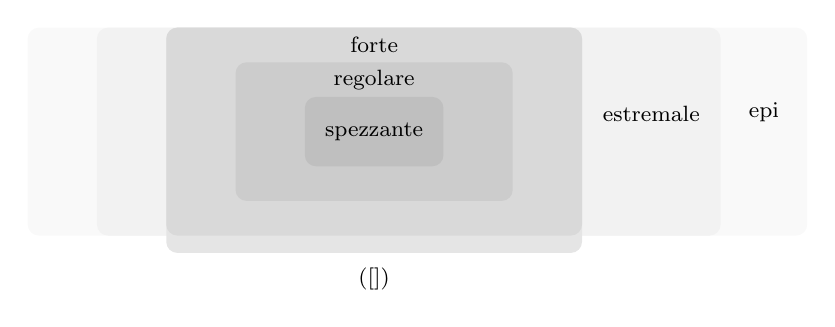
\begin{tikzpicture}[scale=1.1]
			% Outer to inner boxes
			\fill[gray!5,rounded corners] (-4,-1.2) rectangle (5,1.2);
			\node[font=\footnotesize,above] at (4.5,0.0) {epi};

			\fill[gray!10,rounded corners] (-3.2,-1.2) rectangle (4,1.2);
			\node[font=\footnotesize,above] at (3.2,0.0) {estremale};

			\fill[gray!20,rounded corners] (-2.4,-1.4) rectangle (2.4,1.2);
			\node[font=\footnotesize] at (0,-1.7) {$\lort(\Mono[\ctC])$};
			\fill[gray!30,rounded corners] (-2.4,-1.2) rectangle (2.4,1.2);
			\node[font=\footnotesize] at (0,1) {forte};

			\fill[gray!40,rounded corners] (-1.6,-0.8) rectangle (1.6,0.8);
			\node[font=\footnotesize] at (0,0.6) {regolare};

			\fill[gray!50,rounded corners] (-0.8,-0.4) rectangle (0.8,0.4);
			\node[font=\footnotesize] at (0,0) {spezzante};
		\end{tikzpicture}
	\end{center}
	\caption{Gerarchia delle classi di epimorfismi in una categoria \(\ctC\). Le inclusioni si possono invertire sotto le ipotesi indicate. Le classi \(\Epi[\ctC]^s\) degli epi forti di \ref{} e l'ortogonale sinistro \(\lort(\Mono[\ctC])\) sono `essenzialmente sempre' coincidenti nei casi reali, ma \ref{} è un controesempio. Ipotesi opportune su \(\ctC\) rovesciano alcune di queste inclusioni: \Todo{}}\label{fig_gerarchia}
\end{figure}
\subsection{Interazioni tra limiti e colimiti, completamenti}

Interazioni tra limiti e colimiti: commutatività di colimiti filtrati e limiti finiti, commutatività di colimiti setacciati e prodotti. Polinomi (`limiti e colimiti interagiscono per formare un polinomio')

completamenti (il completamento per iniziale è \(\ctC^\lhd\), quello per terminale è il cono destro \(\ctC^\rhd\); descrivere in casi semplici il completamento per prodotti e per coprodotti, gli altri sono più difficili...)

\subsection{Categorie piccolo-complete e piccolo-cocomplete}

\section{Limiti e funtori}
Limiti e colimiti in categorie di funtori. Il caso particolare di limiti in Set (prefasci): per \(F : \ctC^\op\fun\ctSet\), \(\colim F\cong \pi_0(\Elts\ctC F)\). E il limite?

preservazione/riflessione/creazione. criteri di preservazione/riflessione/creazione. esempi.

l'immersione di Yoneda preserva i limiti che esistono nel dominio.



\subsection{}
teorie-prodotto (cioè: teorie algebriche) e teorie-finlimite (cioè: teorie essenzialmente algebriche)

Relazione di yoneda con le teorie limite
\subsection{Coincidenza di limiti e colimiti}
Biprodotti, quadrati esatti in \(\ctAb\)

La definizione di categoria abeliana
\subsection{Proprietà di oggetti specificate da limiti}
Inizialità, finalità (il contenuto della sezione \ref{} su funtori iniziali e finali ora è in contesto), densità (ogni oggetto di \(C\) è colimite di oggetti nella subcat densa) e codensità (più difficile dare un'intuizione, proviamoci)

Oggetti presentabili, oggetti connessi, oggetti minuscoli, oggetti \(\bbD\)-presentabili.





